\chapter{Background \& Literature Overview}
\label{lit review}

The typical multicellular organism stores its genetic code as deoxyribonucleic acid (DNA), found identically in all its somatic cells (unless \textit{de novo} mutations occur). DNA is a biological polymer, consisting of a double-stranded polynucleotide chain. Each nucleotide monomer consists of a phosphate group, deoxyribose (a five-carbon sugar), and one of four nucleobases: adenine (A), cytosine (C), guanine (G), or thymine (T). These two strands are held together with a series of hydrogen bonds between the nucleobases, forming Watson-Crick base pairs. %On opposite strands, adenine and thymine form double hydrogen bonds, while guanine and cytosine form a stronger triple hydrogen bond.

DNA is just the general starting point in a series of information transfers described by the \textit{Central Dogma of Molecular Biology}, which the cell uses to ultimately produce its molecular products \citep{cobb201760}. Through the process of \textit{transcription}, the code from one strand of DNA is transferred onto a primary ribonucleic acid (RNA) transcript. RNA is similar to DNA except that it is single-stranded, has ribose as its five-carbon sugar and uses the nucleobase \textit{uracil} instead of \textit{thymine}. This primary transcript is modified into ribosomal RNA (rRNA), transfer RNA (tRNA) or messenger RNA (mRNA). All three are involved in \textit{protein synthesis}, although mRNA is especially relevant to this project since the protein sequence can be deduced from the mRNA sequence. These molecular products shape the cell's appearance, define how it interacts with external or internal stimuli, and allows it to perform its intended functions. They give each cell type a characteristic RNA profile which can be measured through RNA-seq. Using this technology, we can detect the presence or absence of certain transcriptomic hallmarks of cancer.

% the intro for this is pretty good: https://www.nature.com/articles/s41368-021-00146-0#:~:text=Bulk%20RNA-seq%20studies%20average%20global,next%20generation%20of%20RNA%20sequencing.

%\clearpage
%\section{Differentiation Pathways in the Haematopoietic System}
%. Acute leukaemia occurs earlier in the differentiation pathway, allowing the blasts to divide more rapidly. \autoref{fig:cell_differentiation} shows the mature cell types that result from myeloid and lymphoid cell lineages, which both share \ac{HSC} as the common progenitor cell type.

\clearpage
\section{Acute Myeloid Leukaemia}

%good resource: https://btep.ccr.cancer.gov/wp-content/uploads/RNA-seq_BETP_2019rev.pdf

\ac{AML} is an aggressive form of cancer of the haematopoietic system (\autoref{fig:cell_differentiation}) which is characterised by its rapid proliferation of myeloblasts. This occurs when undifferentiated myeloid cells acquire mutations which hinder further differentiation but allows for their clonal proliferation \citep{Khwaja2016}. This comes at the expense of the production of their healthy, differentiated counterparts: erythrocytes, platelets and granulocytes \citep{Khwaja2016}. It is an exception to cancers in that it does not form a tumour, which is usually analysed to determine the severity. Instead \ac{AML} is staged according to its subtype and other variables \citep{ACS2018}. It is the most common form of acute leukaemia, with an incidence rate of 4.3 per 100,000 in the United States \citep{Kouchkovsky2016}. One of the main risk factors is age, with a median age of diagnosis of 70 years, and with a slight male predominance \citep{juliusson2009age, Khwaja2016}. Acute myeloid leukaemia is synonymous with acute myelogenous leukemia, acute myelocytic leukemia, or acute nonlymphocytic leukemia.

%Summary of leukaemia: https://www.cancer.net/cancer-types/leukemia-acute-myeloid-aml/introduction

\begin{figure}[!h]
    \centering
    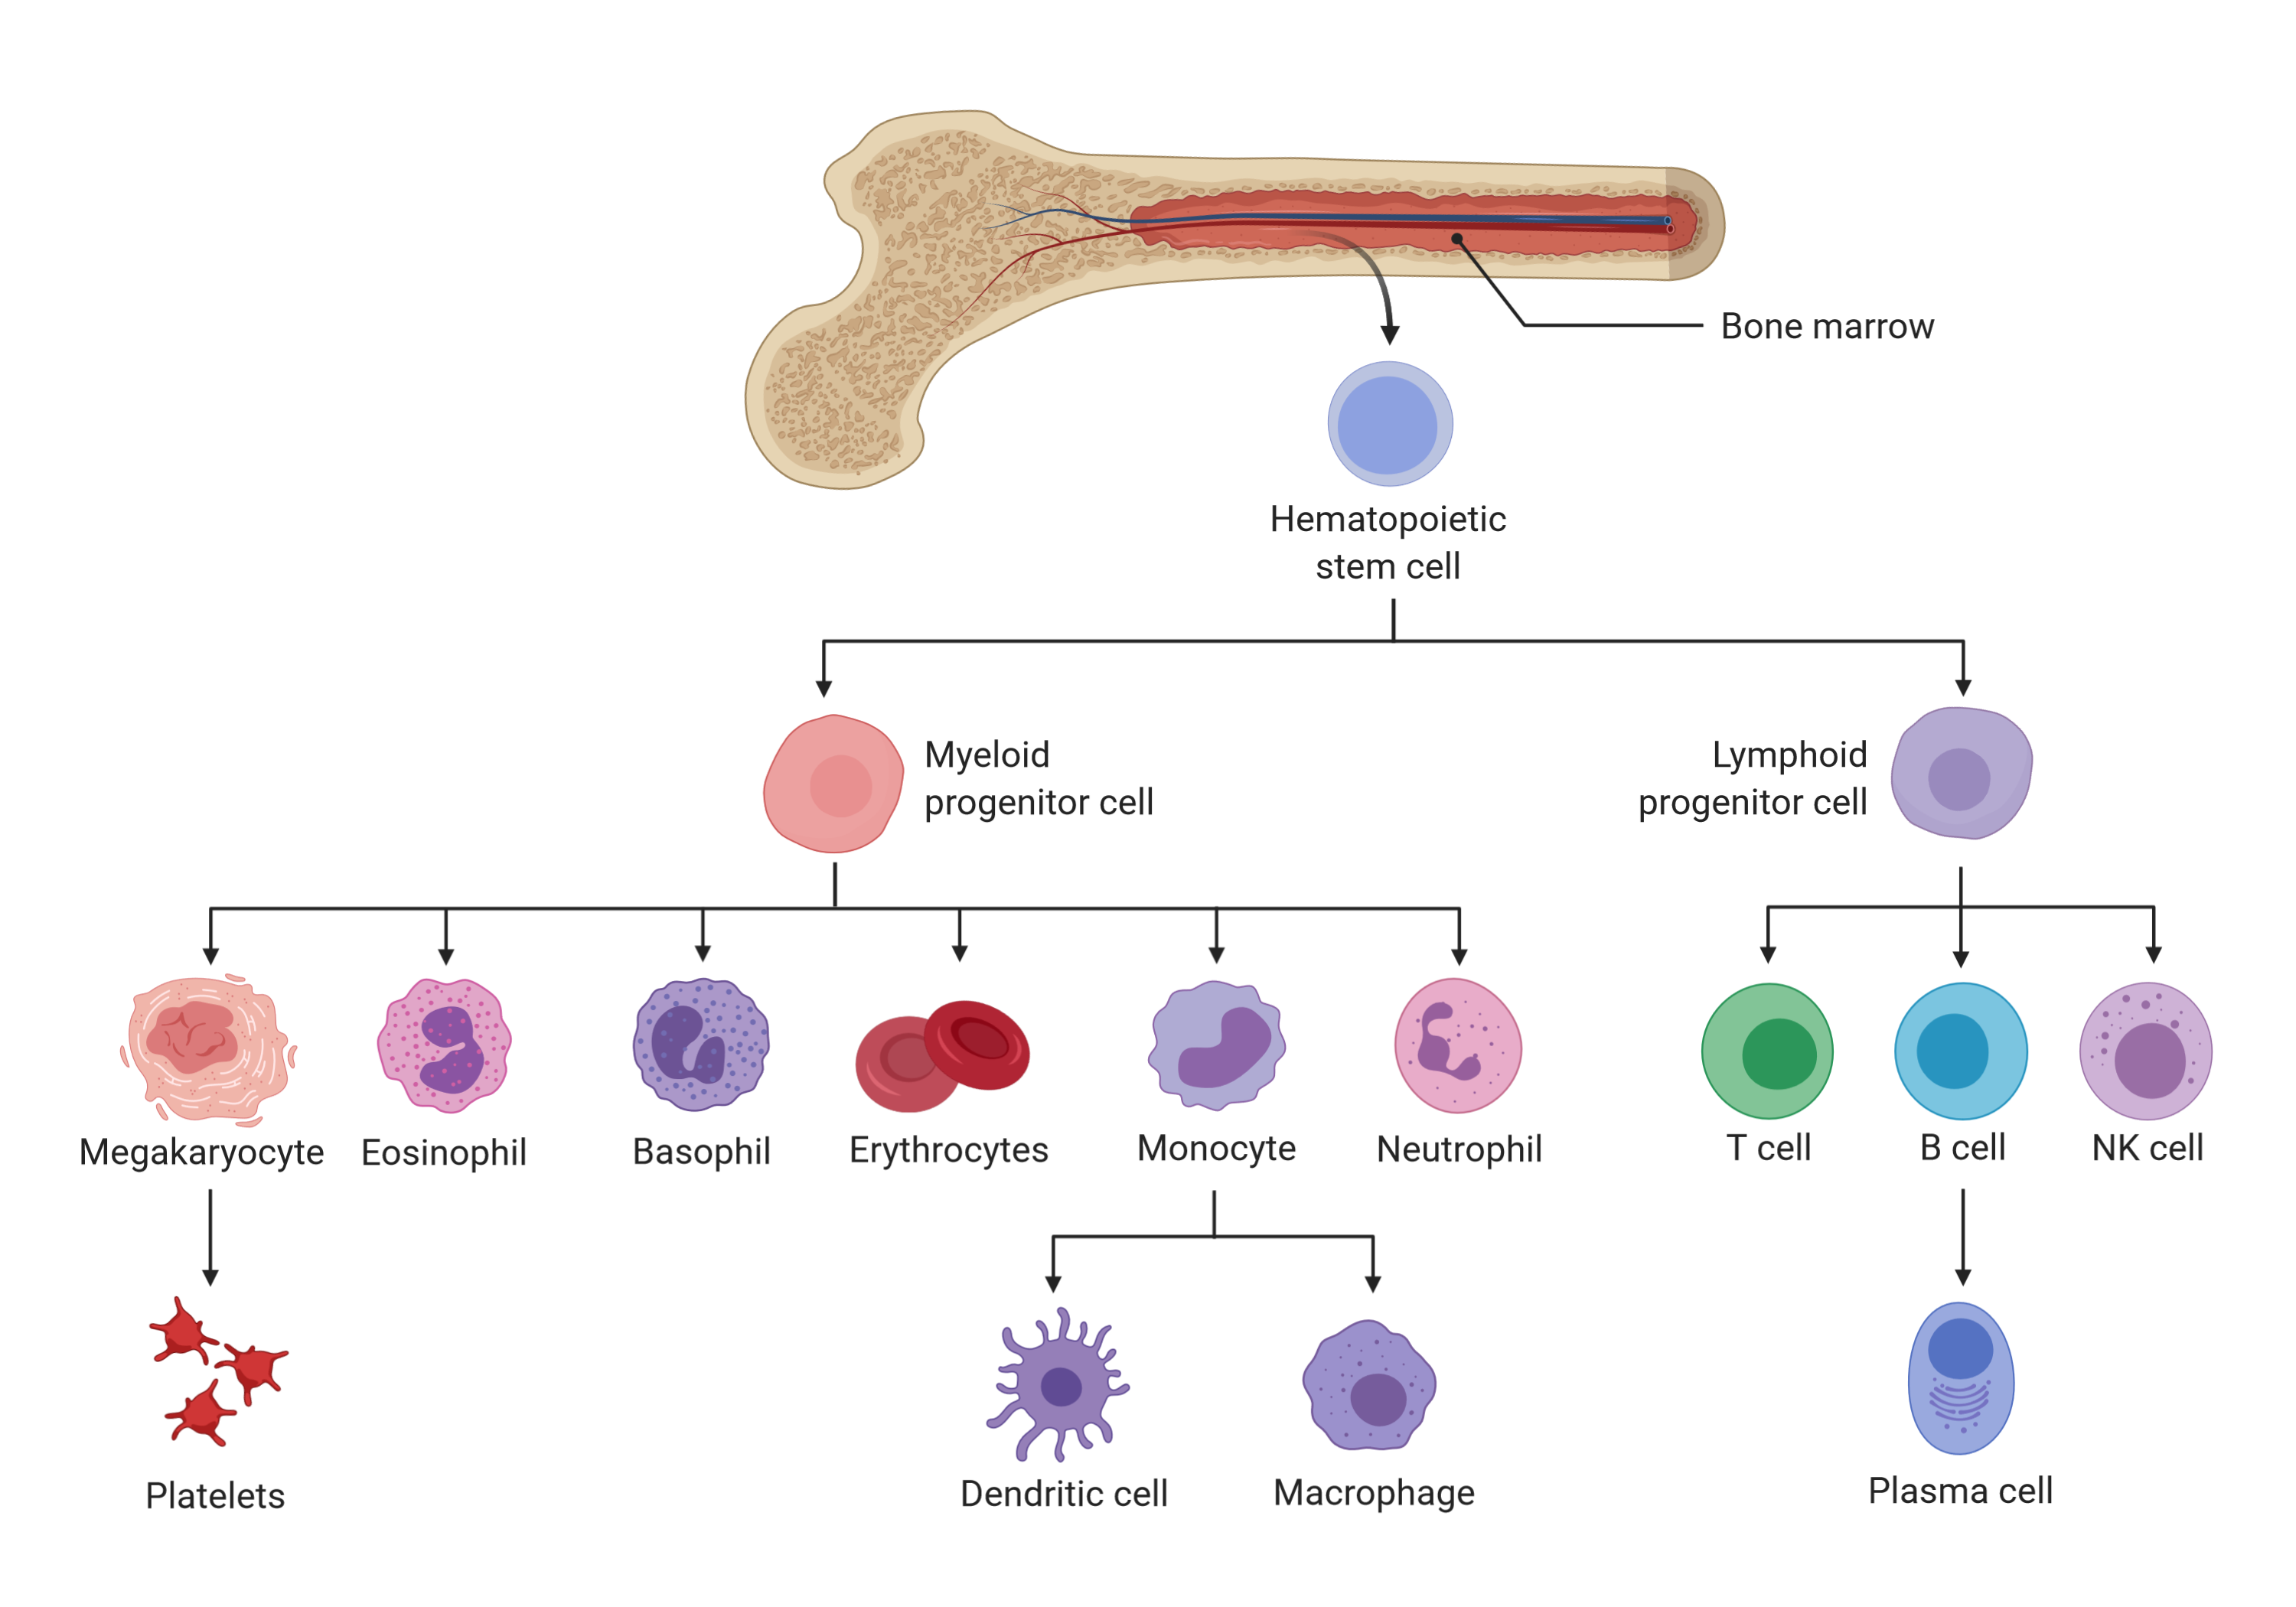
\includegraphics[width=1\textwidth]{cell_differentiation}
    \caption[Stem cell differentiation]{An overview of the main branches of haematopoietic stem cell differentiation pathways showing the myeloid and lymphoid lineages. Created using \href{https://biorender.com/}{BioRender.com}. } 
    \label{fig:cell_differentiation}
\end{figure}

\subsection{Classification and Subtypes}
\label{Classification and Subtypes}
\ac{AML} is one of four main branches of leukaemia classification, the others being Acute Lymphoblastic Leukaemia (ALL), Chronic Myeloid Leukaemia (CML) and Chronic Lymphoblastic Leukaemia (CLL) \citep{leukaemiabook}. Despite their cytogenic differences, there have been multiple reports of chronic leukaemia types transitioning into the more aggressive, acute form over time \citep{kaur2016rapid, frenkel1981acute, jacobs1984acute}. Treatment may vary depending on the subtype of the disease, which is why a rigid classification system and correct identification is important \citep{leukaemiabook}.

Each of these four leukaemia subtypes is subdivided into more specific classifications. \ac{AML} in particular is genetically and morphologically heterogeneous and can involve any single or a combination of myeloid lineages \citep{whoclassification, Kouchkovsky2016}. 

\subsubsection{The FAB classification system}
The \ac{FAB} classification, first produced in 1976, was an early attempt to distinguish subtypes of \ac{AML} \citep{bennett1976proposals}. The divisions were based on cell morphology and the relative quantities of myeloblasts and erythroblasts \citep{ACS2018}.

%Maybe lookup cool table latex tutorials to make it nicer (colours maybe?)
\begin{table}[h]
\centering
\caption{The FAB classification of AML.}
\label{tab:FABclassification}
\begin{tabular}{lll}
\hline
M0 & Undifferentiated acute myeloblastic leukemia        &  \\ 
M1 & Acute myeloblastic leukemia with minimal maturation &  \\
M2 & Acute myeloblastic leukemia with maturation         &  \\
M3 & Acute promyelocytic leukemia (APL)                  &  \\
M4 & Acute myelomonocytic leukemia                       &  \\
M5 & Acute monocytic leukemia                            &  \\
M6 & Acute erythroid leukemia                            &  \\
M7 & Acute megakaryoblastic leukemia                     &  \\ \hline
\end{tabular}
\end{table}

% AML categories are extremely heterogeneous, probably due to high genetic diversity

\subsubsection{The WHO classification system}

A more modern, and now more widely used system, is that devised in the \textit{\ac{WHO} Classification of Tumors of Hematopoietic and Lymphoid Tissues}, now in its revised 4th edition \citep{whoclassification}. \ac{AML} is here defined as having >20\% of the cells in the bone marrow being myeloblasts. The \ac{WHO} based their classification on a mixture of genetic, morphological and cytochemical criteria and based on the presence of other conditions. They define seven subcategories:

\begin{enumerate} \itemsep-0.5em
\item AML with recurrent genetic abnormalities
\item AML with myelodysplasia-related changes (MRC)
\item Therapy-related myeloid neoplasms (t-MN)
\item AML related to previous chemotherapy or radiation
\item Myeloid sarcoma (also known as granulocytic sarcoma or chloroma)
\item Myeloid proliferations related to down syndrome (DS)
\item AML with chromosomal translocations and inversions
\end{enumerate}

These may be further classified according to their specific genetic or karyotypic abnormalities \citep{whoclassification}. Cases which do not fall into any of the above groups, are labelled as 'AML, not otherwise specified (NOS)' and are subject to a form of classification similar to the \ac{FAB} \citep{ACS2018}. Cases classified as having 'recurrent genetic abnormalities' are often sub-categorised and described according their their abnormality (similar to Table \ref{tab:karyotype}, although not all are officially recognised as 'recurring abnormalities').

%https://emedicine.medscape.com/article/2006750-overview?reg=1
%https://www.ncbi.nlm.nih.gov/books/NBK560490/

\subsection{Pathogenesis}
\label{Pathogenesis}
The genetic abnormalities leading to \ac{AML} are heterogeneous and complex, meaning that there are many different combinations of causative genetic or cytogenetic abnormalities which may lead to the \ac{AML} phenotype \citep{lindsley2015acute, whoclassification}. The genetic and karyotypic profile can have profound prognostic impact, affecting both therapeutic strategy and survival rate \citep{mrozek2000prognostic, whoclassification}. 

\subsubsection{Cytogenic Abnormalities}
Approximately 55\% of \ac{AML} patients have at least one cytogenic abnormality \citep{meyer2014translational}.  \cite{stolzel2016karyotype} note that patients with 3 unrelated cytogenic abnormalities, have a worse overall survival rate than \ac{AML} patients with a normal karyotype, and that the patients at most risk had $ \geq $4 unrelated cytogenic abnormalities. There are some exceptions, where the presence of certain abnormalities actually \textit{increases} survival rate with good response to treatment (Table \ref{tab:karyotype}). 

\begin{landscape}
	\pagestyle{empty} % to remove headers on the side	
\begin{table}[h]

    \centering
    \caption{Recurrent abnormalities in AML and their effects. This table makes use of the International System for Human Cytogenomic Nomenclature (ISCN) to describe chromosomal abnormalities \citep{ISCN}. The information given prior to the parentheses denotes the type of chromosomal abnormality (for example \textit{t} for translocation, and \textit{inv} for inversion). The contents of the first pair of parenthesis refer to the affected chromosome(s). The second pair of parentheses, if present, refers to the specific part of the respective chromosome(s) affected (the short arm \textit{p} or the long arm \textit{q}, and which region or band of these arms).}
    \label{tab:karyotype}
    \begin{tabular}{lllllllllllll}
    \toprule
        \textbf{Aberration} & \textbf{Prognosis} & \textbf{Fusion Genes} & \textbf{Note} & \textbf{Reference}  & ~ \\ \midrule
        t(8;21)(q22;q22) & Favourable & RUNX1, RUNX1T1 & Common (\textasciitilde 5\% of all AML) & \cite{reikvam2011acute}  & ~ \\ 
        ~ & ~ & ~ & ~ & \cite{peterson20048}  & ~ \\ \hline
        inv(16)(p13;q22) & Favourable & CBFB, MHY11 & Common & \cite{plantier1994inv}  & ~ \\ 
        t(16;16)(p13;q22) & ~ & ~ & ~ & \cite{shigesada2004mechanism}  & ~ \\ \hline
        t(15;17)(q24;q21) & Favourable & PML, RARA  & Common (\textasciitilde 10\% of adult AML) & \cite{de2014rara}  & ~ \\ 
        ~ & ~ & ~ & ~ &   & ~ \\ \hline
        t(9;11)(p22;q23) & Poor & KMT2A, MLLT3 & Frequency decreases with age & \cite{chandra2010acute}  & ~ \\ 
        ~ & ~ & ~ & ~ & \cite{metzler2004emergence}  & ~ \\ \hline
        t(6;9)(p23;q34) & Poor & DEK, CAN/NUP214 & Rare, associated with an internal tandem & \cite{chi2008acute}  & ~ \\ 
        ~ & ~ & ~ &  duplication (ITD) mutation on FLT3 &   & ~ \\ \hline
        inv(3)(q21.3;q26.2) & Poor & RPN1, MECOM & Rare, low response to standard  & \cite{sitges2020acute} & ~ \\ 
        t(3;3)(q21.3;q26.2) & ~ & ~ & chemotherapy & ~ & ~ \\ \hline
        t(1;22) (p13;q13) & Poor & RBM15, MKL1 & Rare, almost exclusively found in infants   & \cite{carroll1991t} & ~ \\ 
        ~ & ~ & ~ &  with acute megakaryocytic leukaemia & \cite{bernstein2000nineteen} & ~ \\ \hline
        Monosomy  & Very poor & / & Loss of chromosome, frequency increases & \cite{breems2008monosomal} & ~ \\ 
        ~ & ~ & ~ &  with age &   & ~ \\ \bottomrule
    \end{tabular}
\end{table}
\end{landscape}


%t(8;21) is a frequently oc­curring aberration in acute AML. It involves the fusion of the RUNX1 (runt-related transcription factor 1) gene on chromosome 21q22 and the RUNX1T1 (runt-related transcription factor 1; translocated to 1) gene on chromosome 8q22, resulting in the formation of the hybrid gene RUNX1/RUNX1T1. AML with t(8;21)(q22;q22), RUNX1/RUNX1T1 generally shows maturation in the myeloid lineage and is found in approximately 5\% of cases of AML. cite:https://atlasgeneticsoncology.org/haematological/1019/t(8;21)(q22;q22)-runx1-runx1t1

% SUMMARY OF CHROMOSOMAL TRANSLOCATIONS AND THEIR OUTCOMES: https://www.cancer.org/cancer/acute-myeloid-leukemia/detection-diagnosis-staging/how-classified.html


\subsubsection{Genetic Abnormalities}

If we reduce our frame of reference to the genetic level, we find that the aforementioned structural variants (Table \ref{tab:karyotype}) can trigger the activation of an \textit{oncogene}, or their fusion products (Table \ref{tab:karyotype}) can become an oncogene themselves. Some genes have the potential to cause cancer under abnormal conditions and are called \textit{proto-oncogenes}, and if said conditions are met, become the carcinogenic oncogenes. This carcinogenicity can be triggered by either a structural variant, a \ac{SNP} or gene amplification \citep{tabin1982mechanism}. This can cause up-regulation, over-activity or a change in function of the respective protein \citep{tabin1982mechanism}. These proteins are often the targets of cancer drugs \citep{liu2004new}.

Cells have evolved mechanisms to prevent carcinogenesis, through \textit{tumour suppressor genes}. These genes are typically involved in the regulation of cell division, DNA repair or induction of apoptosis. While proto-oncogenes require their up-regulation to induce cancer, tumour suppressor genes require down-regulation or complete deactivation. \cite{knudson1971mutation} suggested a 'two-hit hypothesis', that most tumour suppressor genes require the deactivation of both alleles for carcinogenesis to occur. Knudson theorised that early onset retinoblastoma (cancer of the retina) was caused by an inherited mutation (the first 'hit') and a second acquired mutation (the second 'hit'). Knudson explained late-onset of the disease as being non-inherited, with both 'hits' being acquired. 

%The TP53 gene is the most frequently mutated gene (>50%) in human cancer, indicating that the TP53 gene plays a crucial role in preventing cancer formation.[6] https://doi.org/10.2147%2FOTT.S53876
\clearpage
\begin{table}[H]
    \centering
    \caption{Recurring genetic abnormalities in \ac{AML}. Compiled and adapted from \cite{dinardo2016mutations} and \cite{lindsley2015acute}.}
	\label{tab:genetic abnormalities}
    \begin{tabular}{llllllllll}
    \toprule
\textbf{Role} & \textbf{Role description} & \textbf{Mutated genes} &  &  \\ \midrule
Signalling pathways & Internal or external & NRAS, KRAS, PTPN11, &  &  \\
 & chemical communication & NF1, CBL, KIT, FLT3 &  &  \\ \hline
DNA methylation & Epigenetic modifier, adds & DNMT3A, TET2, IDH1, &  &  \\
 & methyl groups to DNA & IDH2 &  &  \\ \hline
Chromatin modifiers & Epigenetic modifier, & ASXL1, EZH2, BCOR &  &  \\
 & remodels chromatin &  &  &  \\ \hline
Transcription factors & Involved in transcribing & CEBPA, RUNX1, GATA2 &  &  \\
 & DNA into RNA &  &  &  \\ \hline
Tumour suppressors & DNA repair, initiation of & TP53 &  &  \\
 & apoptosis, halting cell growth &  &  &  \\ \hline
Spliceosome complex & Ribonucleoprotein complex & SRSF2, U2AF1, SF3B1, &  &  \\
 & involved in splicing RNA & ZRSR2 &  &  \\ \hline
Cohesin complex & Protein complex involved in & STAG2, SMC3, SMC1A, &  &  \\
 & chromatid cohesion & RAD21 &  &  \\ \hline
Others & Other proto-oncogenes & WT1, PHF6, TP53, &  &  \\
 &  & NPM1 &  &  \\ \bottomrule
    \end{tabular}
\end{table}

%\subsection{Transcriptomic abnormalities}
%Pathways

\subsection{ Treatment Methods}
\label{Treatment Methods}
Surgery, chemotherapy, radiotherapy, immunotherapy and hormone therapy are common treatments used to kill cancer cells. While the specifics are partly dependent on the particular \ac{AML} subtype and the patient's condition, some variation of chemotherapy is standard practice. Treatment is typically split into four phases spread over a period of 2-3 years \citep{malard2020acute}:  

\begin{enumerate}
\item \textbf{Induction}\hspace{0.2cm}Uses chemotherapeutic drugs with the intention of achieving complete remission (no symptoms or signs of cancer) and restore normal cellular activity. Cytarabine (AraC) is one of the most commonly used chemotherapeutic drugs for \ac{AML}, often used in conjunction with others such as daunorubicin \citep{Robak2009}.
\item \textbf{Consolidation}\hspace{0.2cm}Consists of several short sequential courses of chemotherapy every two weeks, usually using stronger doses.
\item \textbf{Intensification}\hspace{0.2cm}Also called reinduction therapy, includes drugs similar to those used during the induction phase.
\item \textbf{Long-term maintenance}\hspace{0.2cm}Chemotherapy is performed for 2-3 years after complete remission to prevent, or slow down, the growth of any cancer remnants. At times, a bone marrow or stem cell transplant is sometimes necessary to replenish the supply of healthy hematopoietic cells
\end{enumerate}

In recent decades, advances in our knowledge of cancer biology and the development of more efficient high-throughput sequencing techniques, have lead to the identification of novel treatments which specifically target cancer cells, such as differentiation therapy. A key characteristic of cancer cells is remaining in a stem-cell like state, which allows for their rapid proliferation. Differentiation therapy is a relatively modern approach which attempts to induce the process of differentiation, where the malignant cells mature and lose their ability to proliferate, rendering them virtually harmless. The first successful differentiation agent was \ac{ATRA}, also known as tretinoin, used to treat acute promyelocytic leukaemia (APL) \citep{chomienne1990all}. This revolutionary drug managed to achieve a 90\% survival rate in APL patients, without the severe cytotoxic side-effects of traditional non-targeted chemotherapy \citep{kim2015selection}. There have been many attempts to emulate this with other compounds, with mixed results \citep{nowak2009differentiation}.

\subsection{The Model Cell Line: HL-60 }
A 36-year-old Caucasian woman was being treated for \ac{AML} at the MD Anderson Cancer Center in Texas, 1977, when she consented to being part of a study on her disease. Researchers took a blood sample, from which they extracted blasts for their analysis. Three years later, \cite{gallagher1979characterization} would describe for the first time the HL-60 cell line, now one of the most widely used \ac{AML} cell lines. The cells were described as having primarily neutrophilic and promyelocytic morphology, and thus initially placed into the \ac{FAB}-M3 'acute promyelocytic leukemia' category (see Section \ref{Classification and Subtypes}). Subsequent analysis of the cells' karyotype, performed by \cite{dalton1988hl}, revealed that they lacked the t(15;17) translocation characteristic of \ac{FAB}-M3, and were categorised as \ac{FAB}-M2, but development in nomenclature led the cell-line to finally being placed in the 'AML with maturation' category, using the \ac{WHO} system.

Early karyotypic studies had identified the t(5;17) \citep{von1990double} and t(9;14) translocations, together with a complex structural variant between chromosomes 5, 7, and 16 \citep{liang1999spectral}. A more recent study by \cite{jacobson2020hi} used genome wide chromatin conformation capture (Hi-C) and RNA-seq to study structural variants in HL-60 genetic branches. They have shown the heterogeneity in HL-60 cell lines, but identified novel structural variants thought to be found in the original HL-60 sample: t(5;7)(q31.2;q32.3), t(5;16)(q33.3;q23.2-q23.3), t(7;16)(q32.3;q24.1), t(9;14)(q31.1;q23.2), and t(5;17)(q11.2;p11.2).

As mentioned in Section \ref{Treatment Methods}, \ac{ATRA} has been a success story in \ac{AML} differentiation therapy, and since its discovery, has been extensively used on HL-60 cells. This has led to the evolution of an ATRA-resistant branch of the HL-60 cell line, which was used during the study \citep{Gatt2016} that laid the foundation for this dissertation. \cite{fu2005effects} were successful in reverting this resistance through gene knockdown of MCL-1, which seems to produce the protein responsible for \ac{ATRA} resistance.

%Pathway analysis
%Read Lucienne's papers and their references

\clearpage
\section{RNA-seq: \textit{in vitro}}
RNA sequencing (RNA-seq) is the application of a \ac{NGS} technique to measure the quantity of RNA sequences in a biological sample, in a given moment \citep{zhong2009}. Since its first publications in 2008 \citep{nagalakshmi2008transcriptional, lister2008highly, cloonan2008stem}, RNA-seq has gradually been replacing microarrays as the standard technology in molecular biology to analyse \ac{DGE}. Its main advantage is that it allows for the sequencing of the entire transcriptome, while microarrays only allow for predefined regions to be sequenced \citep{rao2019comparison}. 

Sanger sequencing is considered as the first generation in a series of changes in sequencing technology, developed in 1977 and dominated the nucleic acid sequencing industry for over 30 years \citep{behjati2013next}. Next-generation sequencing (or second generation sequencing) revolutionised the industry, its massively parallel capabilities allowing for greatly increased throughput, sequencing millions of fragments at a time instead of Sanger sequencing's just one. At the time of writing, we are currently in the process of transitioning into the third generation of nucleic acid sequencing, which allows for longer reads (>1000 bp as opposed to 35-600 bp). Longer reads translate to greater overlap between the reads, and thus greater certainty during assembly or alignment, particularly when considering regions of low-complexity or structural variants \citep{rhoads2015pacbio}. 

We should make a distinction between two popular types of RNA-seq: the classic bulk RNA-seq, and single-cell RNA-seq (scRNA-seq). Bulk RNA-seq, which this project has made use of, takes the average gene expression of a sample, which may be composed of many cell types, while scRNA-seq investigates the transcriptome of each individual cell. RNA-seq is traditionally used to profile transcriptomes, but it may be used in the identification of expressed SNPs, identification of novel transcripts, the detection of fused genes and alternative splicing \citep{han2015alternative, zhao2014comparison}. 

The following section is an overview of the techniques used to transform the nucleotide sequences residing inside living cells into letters on a screen. While this project deals with the data analysis part of RNA-seq, some background on the origins of said data is essential. 

% great summary of rna sequencing: https://www.sciencedirect.com/science/article/pii/S0090825818312836#bb0080
% also really good https://www.thieme-connect.com/products/ejournals/html/10.1055/s-0039-1688446

\subsection{Experimental Design}

%https://genomebiology.biomedcentral.com/articles/10.1186/s13059-015-0697-y: 
%https://www.ncbi.nlm.nih.gov/pmc/articles/PMC4878611/

An RNA-seq experiment is customised according to research goals and often limited by the budget. Since many of the following options are an accuracy/expense trade-off, the researcher should be knowledgeable on the options to effectively allocate funds, particularly if the sequencing will be outsourced to another company. This section was placed here to retain the chronological order in which an RNA-seq experiment would take place, although some of the below descriptions include some technical detail which will be explained in future sections.

\begin{itemize}

\item[] \textbf{Read length} \hspace{0.15cm} Before sequencing, it is possible to specify the number of base-pairs of the DNA fragments each read would contain. A distinction is made between reads which emerge from second-generation sequencing machines (short-reads) and third-generation sequencing machines (long-reads). Smaller reads lead to greater ambiguity during alignment as they have a greater probability of being multi-mapped, and partly determine the optimal alignment algorithm \citep{albert2020biostar}. This is especially true in regions of low-complexity or in the presence of structural variants \citep{rhoads2015pacbio}. The exception to this rule is in the study of small RNAs, where read lengths drop to <30bp \citep{albert2020biostar}.

\item[] \textbf{Depth of coverage} \hspace{0.15cm} Coverage is the average number of reads that will cover a given sequence, meaning that it is determined by the read length and number of reads. It is commonly denoted with an \textit{x}, e.g. 30x coverage means that a nucleotide is covered by an average of 30 reads. Low coverage is susceptible to ambiguity and sequencing errors.

\item[] \textbf{Paired-end reads} \hspace{0.15cm} Fragments of cDNA are typically longer than the read length, so some sequencing information may be lost. Paired-end sequencing, as opposed to single-end sequencing, allows both ends of the cDNA fragment to be sequenced. The distance between each paired-end read is known, which is fed into alignment algorithms that use this information to improve alignment. This especially improves regions of low complexity \citep{albert2020biostar}.

\item[] \textbf{Sample replicates} \hspace{0.15cm} Technical replicates originate from the same biological source to produce multiple samples which are all processed in the same manner. This gives isolates the non-biological variation, allowing for the evaluation of the instruments and methodology used. By contrast, biological replicates originate from different biological sources and are meant to test the biological variance of the samples. A mixture of the two types may be used, however given a limited budget, biological replicates are preferred in RNA-seq because technical variation is minimal \citep{bullard2010evaluation}, by far outweighed by biological variation \citep{liu2014rna}. \cite{schurch2016many} found that using three biological replicates gave 20\% to 40\% of the \ac{DEG}s (varies according to the tool) compared to a full set of 42 replicates (representing the 'true' population). This rises to >85\% when considering genes with a log$_2$ fold change of >2.
\end{itemize}


\subsection{RNA extraction}
The first step in any RNA-seq workflow is the extraction of RNA from the biological sample. This is complicated by the chemical instability of RNA due to its hydroxyl groups at the 2' and 3' positions, facilitating RNase activity (RNA-degrading enzymes) \citep{green2019win}. This issue is compounded by the ubiquity and chemical resilience of RNAses, meaning that special care must be taken to avoid contamination of glassware and instruments that interact with the RNA \citep{green2019win}. One method uses liquid nitrogen to deactivate any RNase enzymes and freeze the samples, which are pulverised to extrude the cell contents \citep{wang1994extraction}. 

The data serving as the basis for this dissertation was provided by \cite{Gatt2016}, who followed the RNeasy® Mini kit \citep{RNeasy} which makes use of an extraction technique called \textit{acid guanidinium thiocyanate-phenol-chloroform} (AGPC) extraction \citep{chomczynski1987single}. This is based on \ac{LLE} \citep{mazzola2008liquid}, where under acidic conditions the cell's RNA partitions into the aqueous phase while the DNA, proteins and lipids partition into the organic phase, aided by centrifugation. The organic phase is composed of phenol (which dissolves the protein) and chloroform (which dissolves the lipids). Guanidinium thiocyanate is part of the kit's buffer solution, and acts as a chaotropic agent, meaning it disrupts water's hydrogen bonds. This is added to the organic phase to disrupt the hydrophobic properties of protein (including RNases), aiding in their denaturation. Ethanol is added to precipitate the RNA and any residual DNA. A spin-column is used to bind nucleic acids to a silica membrane, and wash away any proteins, carbohydrates, fatty acids and any traces of salts, aided by centrifugation \citep{matson2009microarray}. The end-result is a purified aqueous nucleic acid solution. 

RNA concentration is commonly checked through quantitation using a spectrophotometer, which measures the ability of the sample to absorb UV light at wavelengths of 260nm and 280nm. A score is assigned to the sample's ability to absorb each of the two wavelengths, and the purity of the sample is often quantified using the ratio between the two scores (A260/280 ratio). A pure RNA sample should yield an A260/280 ratio of ~2.0 \citep{scientific2013t042}.

An additional quality metric commonly checked before sequencing, is the integrity of the RNA. This can be quantified via the \ac{RIN} algorithm, applied to the results of capillary electrophorisis, which separates the RNA fragments based on their length \citep{schroeder2006rin}. In most labs, the electrophoresis and computation of the \ac{RIN} is performed automatically in an electropherogram \citep{chamieh2015quantitative}. A poor \ac{RIN} may indicate RNase contamination during extraction, that could have degraded the RNA.

\subsection{Library Preparation}
'RNA' is a generic term, which includes both coding and non-coding RNA. Ribosomal RNA (rRNA) is a form of non-coding RNA which comprises 80\% to 95\% of the total RNA \citep{o2013ribosomal, kukurba2015rna} and must be removed before sequencing. 

There are two main competing methods available, each with their unique advantages and restraints: poly-A enrichment and rRNA depletion. The 3' end of messenger RNA (mRNA) undergoes polyadenylation prior to transcription, meaning that a long chain of adenine nucleotides called the \textit{poly-A tail} is added. With poly-A enrichment, RNA fragments with a poly-A tail are enriched with oligo (dT) primers, thus selecting for the mRNA \citep{zhao2014comparison}. The alternative approach is an active removal of the rRNA using commercially available kits, such as the Illumina \textit{Ribo-Zero Plus rRNA Depletion Kit}. These kits use oligonucleotides complementary to the rRNA sequences to reduce their abundance \citep{griffith2015informatics, peano2013efficient}. 

The next two steps are fragmentation and conversion to complimentary DNA (cDNA), the order of which may vary. In the Illumina workflow used to generate the data for this dissertation, the RNA strands were first fragmented, and reverse transcribed to their cDNA counterparts \citep{pease2012rapid}. A short, artificially synthesised oligonucleotide called an \textit{adapter} sequence is ligated to each of the cDNA fragments, using the ligase enzyme, together with sequence motifs such as barcode sequences \citep{pease2012rapid} (\autoref{fig:ngs_clonal_amp}).

%This adapter-ligated cDNA library is typically attached to a flow-cell, amplified and sequenced in a high-throughput sequencing platform which typically results in a FASTQ \citep{cock2010sanger} file. % Include more detail here?

%cDNA synthesis and preparation 
%of an adaptor-ligated sequencing library. The library is 
%then sequenced to a read depth of 10–30 million reads 
%per sample on a high-throughput platform (usually 
%Illumina)

\begin{figure}[!h]
    \centering
    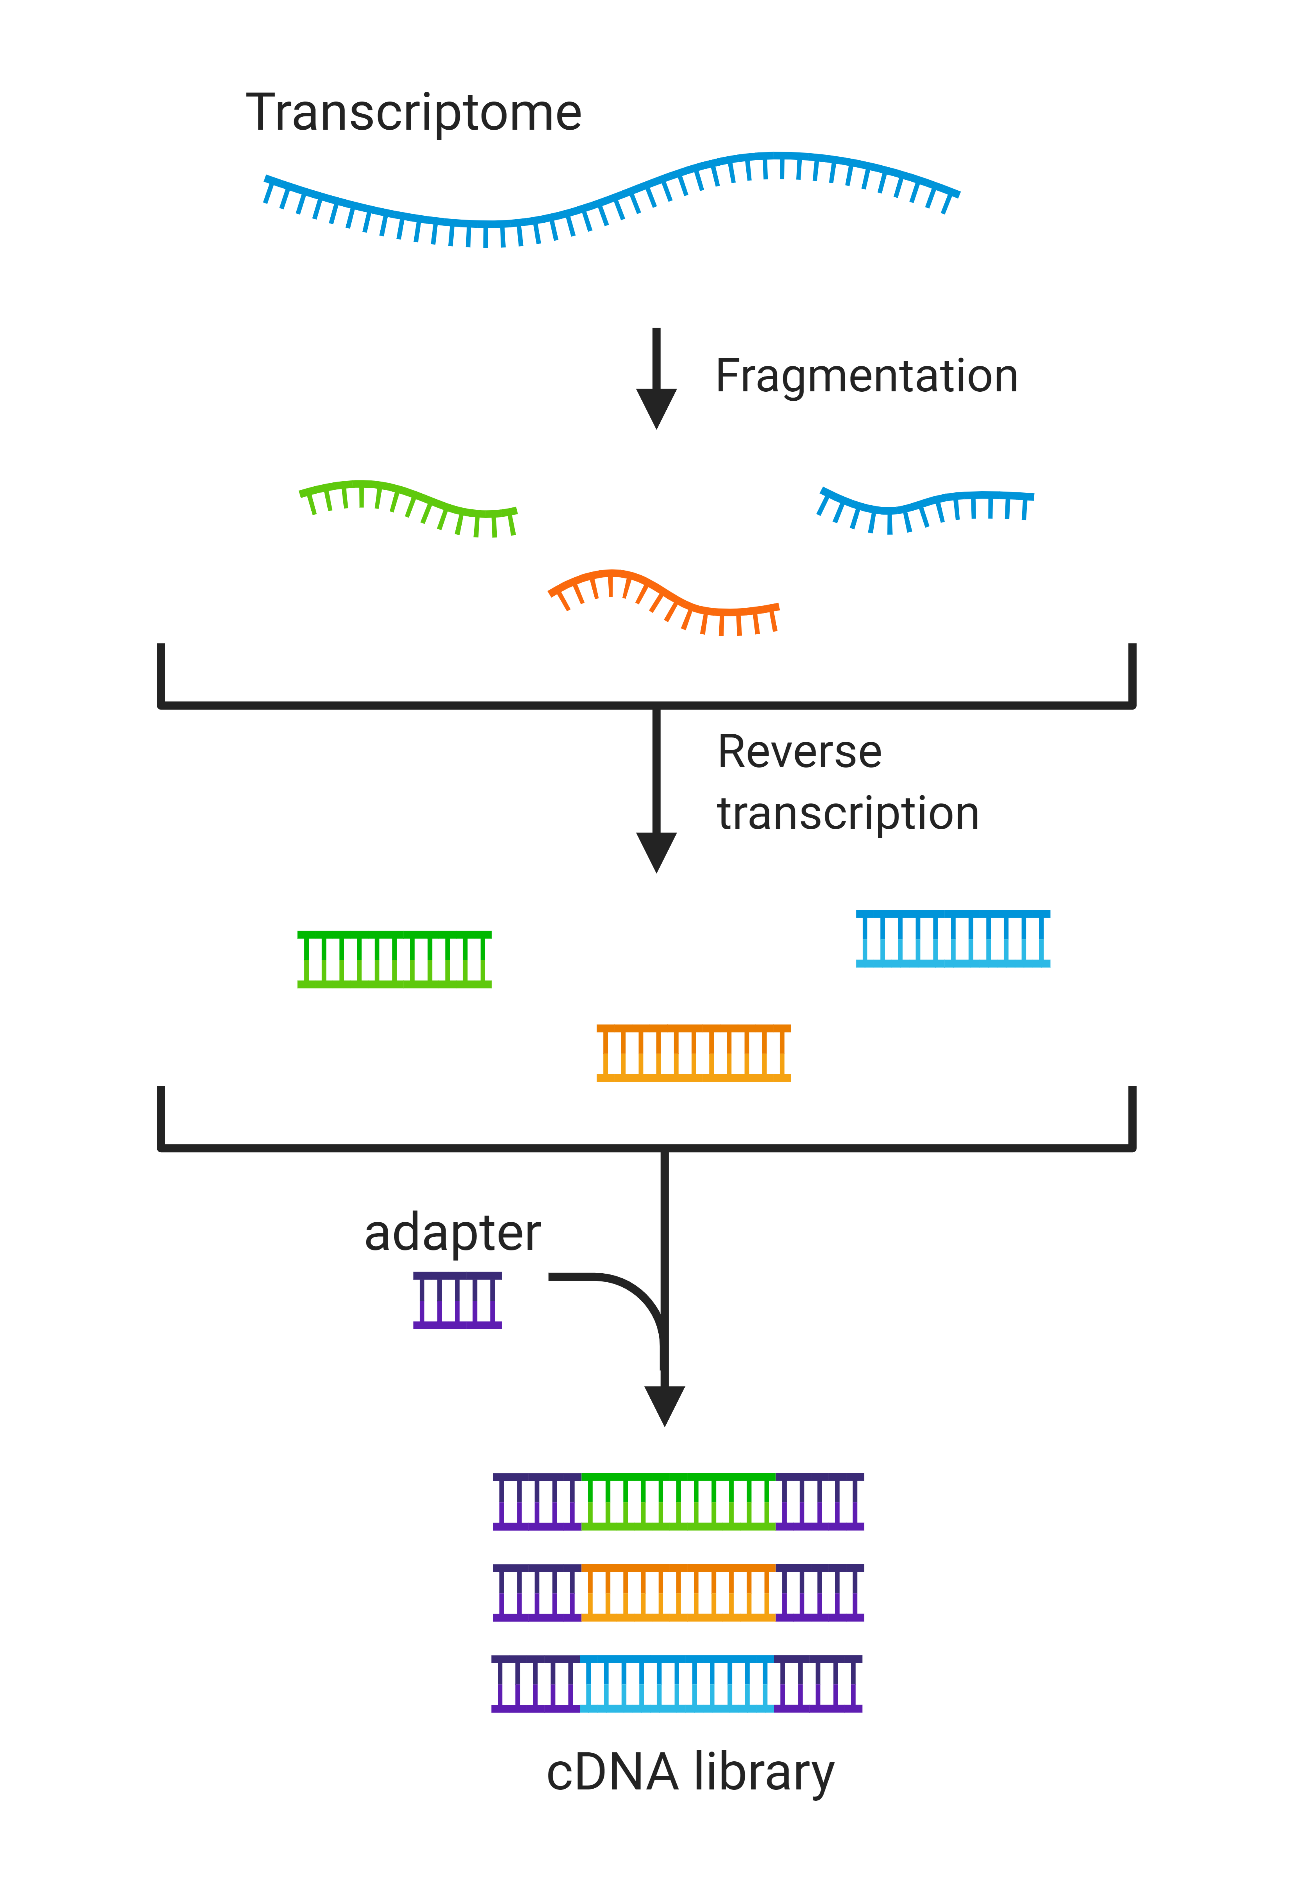
\includegraphics[width=8cm]{ngs_lib_prep}
    \caption[Library preparation]{Illumina library preparation. Created using \href{https://biorender.com/}{BioRender.com}. } 
    \label{fig:ngs_lib_prep}
\end{figure}
%\clearpage

\subsection{Clonal amplification}
The following step amplifies the fragments of the cDNA library to a level detectable by the sequencing machine, using a form of \ac{PCR}. The Illumina Sequencing by Synthesis technology makes use of the flow-cell-based method of \textit{bridge amplification} \citep{illumina2010}, as opposed to emulsion PCR, a similar technology used in Ion Torrent Semiconductor Sequencing which makes use of bead surfaces \citep{williams2006amplification}.

In bridge amplification \citep{illumina2010}, the previously prepared adapter-ligated cDNA library is attached to a flow cell, which is a hollow glass slide with multiple channels, coated with a lawn of oligonucleotides (called oligos in short) complimentary to the sequences which form part of the adapters. Strands of cDNA bind to these oligos, and polymerase creates the complement of the hybridised strand. Each double-stranded cDNA molecule is then denatured and enters a number of bridge-amplification cycles. Each molecule is amplified, forming clusters of identical cDNA sequences adjacent to each other (\autoref{fig:ngs_clonal_amp}).

\begin{figure}[!h]
    \centering
    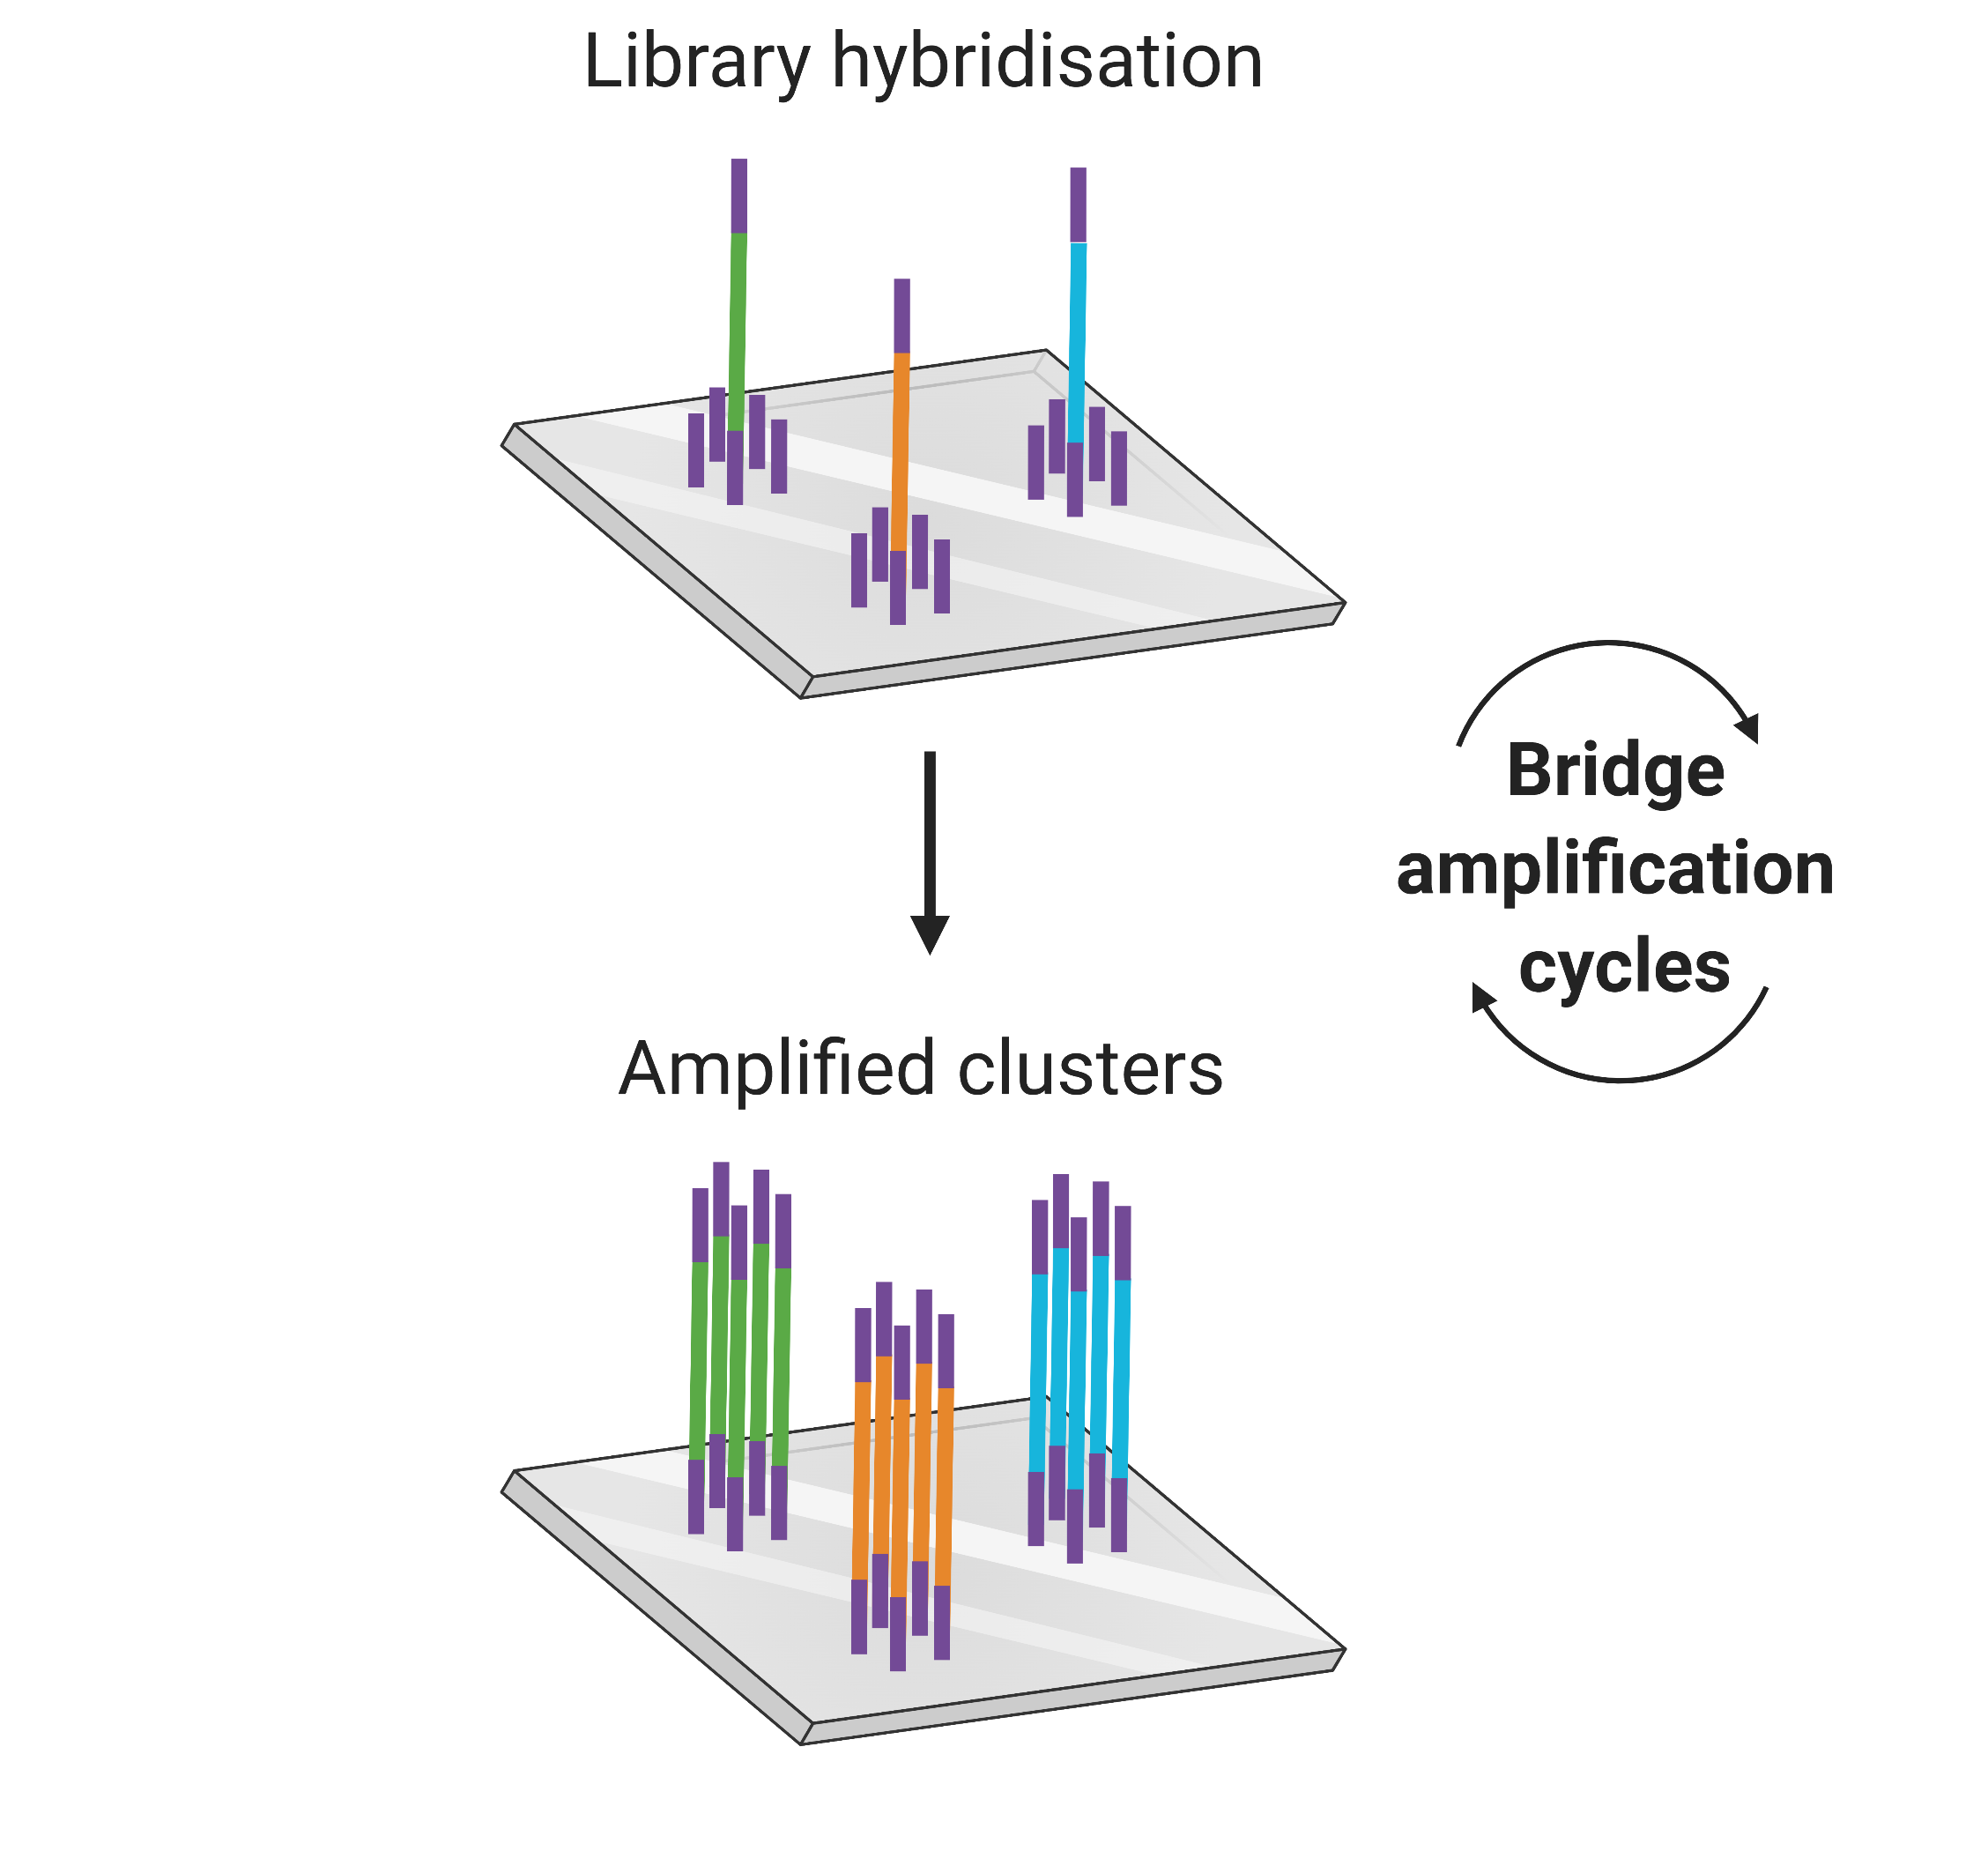
\includegraphics[width=8cm]{ngs_clonal_amp}
    \caption[Illumina clonal amplification]{Illumina clonal amplification. Created using \href{https://biorender.com/}{BioRender.com}. } 
    \label{fig:ngs_clonal_amp}
\end{figure}
%\clearpage

\subsection{Sequencing and Nucleobase Detection}
Sequencing by Synthesis \citep{illumina2010} makes use of fluorescently-labelled deoxynucleoside triphosphate (dNTP). Each sequencing cycle binds a dNTP molecule to the millions of clusters in parallel, with each of the four nucleotides emitting a different coloured light upon binding and laser excitation. The sequencing machine captures the light being emitted from the flow cell as an image and identifies the first base of each fragment. The cycle repeats itself for the second base, third base, and so on, until the end of the sequence (\autoref{fig:ngs_sequencing}). The raw sequencing data is stored as Binary Base Call (BCL) files.

Multiple samples may be sequenced simultaneously during a single run, where they are multiplexed by the machine, meaning they are pooled into a single data stream. Unique identifiers called barcode sequences (added to the cDNA fragments during library preparation) allow for the recognition of the different samples, and demultiplexing of the BCL files into text-based FASTQ files \citep{cock2010sanger}. These are immediately compressed to reduce costs associated with data storage and data transfer. While the \textit{de facto} data compression format used is gzip \citep{deutsch1996gzip}, and bzip is used on occasion \citep{seward1996bzip2}, the underlying compression algorithms used are unspecialised and inefficient for genomic data.

\begin{figure}[!h]
    \centering
    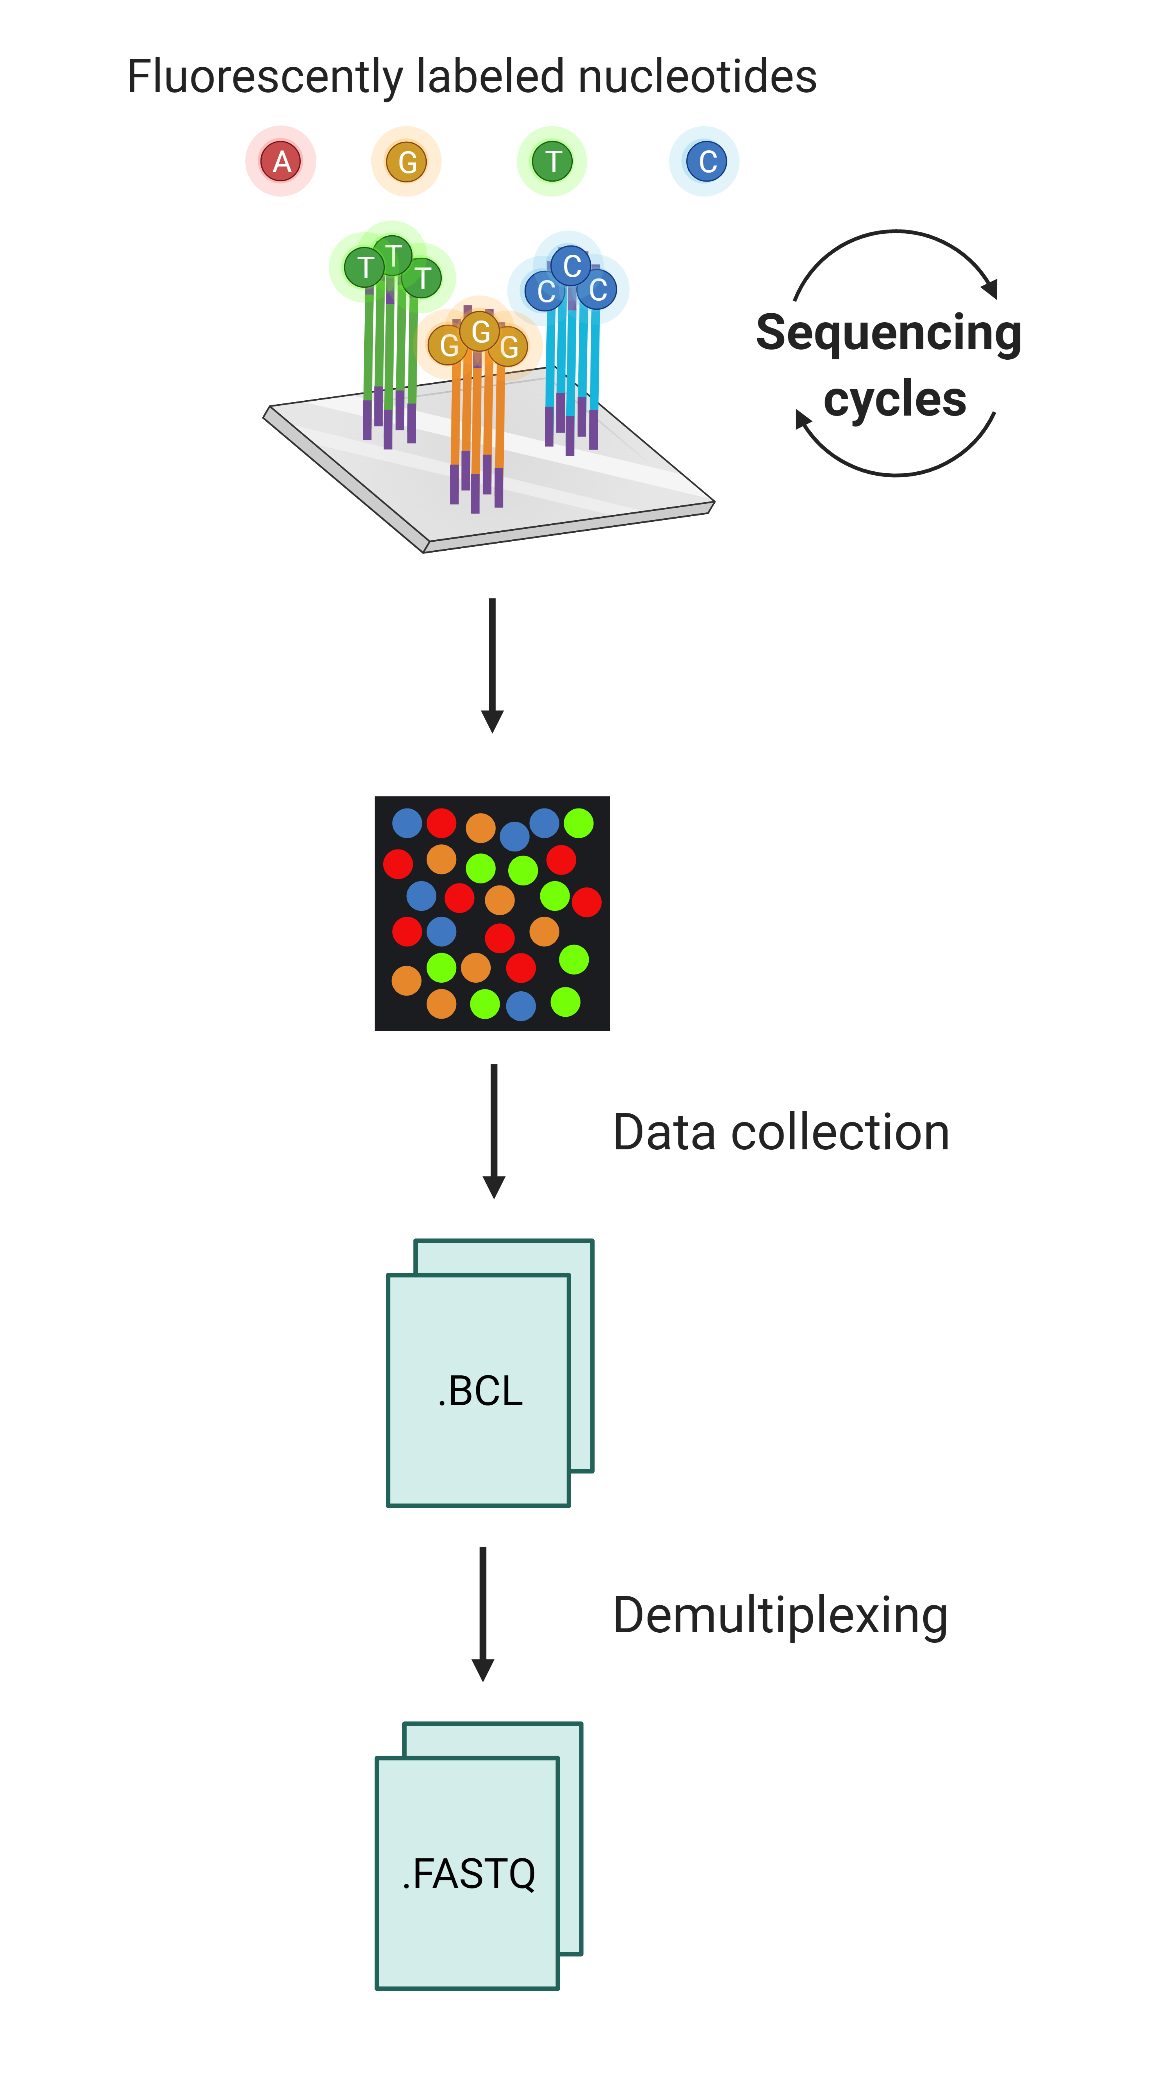
\includegraphics[width=8cm]{ngs_sequencing}
    \caption[Sequencing by synthesis]{Illumina sequencing by synthesis. Created using \href{https://biorender.com/}{BioRender.com}. } 
    \label{fig:ngs_sequencing}
\end{figure}
%%\clearpage

%illumina sequencing steps: https://www.illumina.com/documents/products/techspotlights/techspotlight_sequencing.pdf
% Potential sequencing errors

%Low complexity regions
%Sequencing software which cannot determine the nucleotide in a particular position, often represent the ambiguous base as 'N'. 
%Potential sequencing errors

% paired end vs single end: Paired-end sequencing sequences both the 5’ and 3’ end of each fragment
% read length
% coverage


\clearpage
\section{RNA-seq: \textit{in silico}}
\label{RNA-seq: in silico}

Once the FASTQ files emerge from the sequencing machines, we may move into the dry lab and feed the data into an RNA-seq data analysis pipeline. While the specific tools which make up the pipeline will vary according to the type of data and goals of the researcher, RNA-seq pipelines share a common skeleton. The following subsections will first provide a general overview of the respective step in the pipeline, and then delve into the specific tools used in this project. They were inspired by a multitude of online tutorials and resources, accessed between 29/05/2022 and 10/06/2022:

\begin{itemize}\itemsep-0.5em
\item \url{https://chagall.med.cornell.edu/RNA-seqcourse/}
\item \url{https://training.galaxyproject.org/training-material/topics/transcriptomics/tutorials/rb-RNA-seq/tutorial.html}
\item \url{https://btep.ccr.cancer.gov/wp-content/uploads/RNA-seq_BETP_2019rev.pdf}
\item \url{https://www.bioconductor.org/packages/devel/bioc/vignettes/DEGreport/inst/doc/DEGreport.html}
\item \url{https://training.galaxyproject.org/training-material/topics/sequence-analysis/tutorials/quality-control/tutorial.html}
\item \url{https://chagall.med.cornell.edu/RNA-seqcourse/Intro2RNA-seq.pdf}
\end{itemize}

%Introns are spliced out of the pre-mRNA to form a mature mRNA transcript

\subsection{Quality Control}

The first part of any sequencing pipeline should be to analyse the quality of the data received from the sequencing machine. If poor quality sequencing information is identified, it is truncated to mitigate inaccuracies in the downstream pipeline. Some imperfections and uncertainties in sequencing are unavoidable, thus the reading of each base call by the sequencer is assigned a Phred quality score. These are numerical scores generally ranging from 10 to 60, logarithmically related to the probability of an erroneous base-call, represented as a single ASCII character \citep{ewing1998base}. They are calculated as follows:
$$ Q = -10 log_{10}P $$
 $$P = 10^{\frac{-Q}{10}}$$
 
where:
\begin{conditionsenv*}
	Q 		& Phred-scale quality score \\
	P 		& Probability of an erroneous base call \\
\end{conditionsenv*}

A common convention is to write the value of the Phred score after the letter \textit{Q}, so we may say that a base call with quality of Q30 has a 0.1\% chance of being erroneous. The FASTQ files used for this project are Sanger/Illumina 1.9 encoded, meaning that the assigned character to the score is equal to its value as an ASCII code + 33. So Q30 would correspond to the ASCII character with an ASCII code\footnote{The complete Q-score encoding table: \url{https://support.illumina.com/help/BaseSpace_OLH_009008/Content/Source/Informatics/BS/QualityScoreEncoding_swBS.htm}} of 53, which is the question mark character \textit{?} \citep{ewing1998base}. The lack of a base call is represented as an \textit{N} in place of the nucleotide.

\subsubsection{FastQC}
\begin{itemize}\itemsep-0.5em
\item[] \textbf{Citation}: 				\cite{andrews2010fastqc}
\item[] \textbf{Documentation}: 	\url{https://www.bioinformatics.babraham.ac.uk/projects/fastqc/Help/3\%20Analysis\%20Modules/l}
\item[] \textbf{Dependencies}: Java, Picard BAM/SAM Libraries (included in download)
\end{itemize}
% Useful: https://rtsf.natsci.msu.edu/genomics/tech-notes/fastqc-tutorial-and-faq/#:~:text=FastQC%2C%20written%20by%20Simon%20Andrews,on%20a%20sequence%20data%20set.
In the rapidly changing field of nucleotide sequencing, FastQC has been one of the few constants. It has become a staple quality control tool for high throughput sequencing data, accepting BAM \citep{BAM}, SAM \citep{li2009sequence} or FASTQ files as input, from which it produces an HTML-based report using a number of modules measuring various quality metrics. The software rates each of these modules using a green check-mark signifying that it 'passed' QC, a yellow exclamation mark 'warning', or a red cross 'failed'. However these flags are set to DNA sequencing standards, and have limited applicability with other types of sequencing, such as RNA-seq, where a number are expected to fail \citep{fastqctutorial2021}. These modules are thoroughly described in its documentation and summarised below. Care should be taken as the X-axis is non-uniform for a number of the produced graphs.

%Maybe add expected moduels to fail
\begin{itemize} \itemsep0em
\item[] \textbf{Modules used in FastQC:}
\item \textbf{Basic Statistics} \hspace{0.2cm} Some basic information on the file: its name, type of quality score, total read count, read length and GC content.
\item \textbf{Per Base Sequence Quality} \hspace{0.2cm} The aggregated Q-scores at each position of the reads, represented by a box-plot.
\item \textbf{Per Sequence Quality Scores} \hspace{0.2cm} The number of reads on the Y-axis and the average Q-score on the X-axis.
\item \textbf{Per Base Sequence Content} \hspace{0.2cm} A relative abundance line graph showing the percentage abundance of each of the four nucleotides across all the reads. 
\item \textbf{Per sequence GC content} \hspace{0.2cm} The percentage abundance of each of the four nucleotides across all the reads, overlaid on the expected distribution. 
\item \textbf{Per base \textit{N} content} \hspace{0.2cm} Percentage of bases at each position of the sequence with no base call, represented as an \textit{N}.
\item \textbf{Sequence Length Distribution}\hspace{0.2cm} Shows the distribution of sequence lengths, measured in number of base-pairs (bp). The module will raise a warning if all sequences are not the same length and an error if any of the sequences have zero length.
\item \textbf{Sequence Duplication Levels} \hspace{0.2cm} Percentage of reads in the library which come from sequences with duplication. Two lines indicate the percentages of the raw and the deduplicated libraries.
\item \textbf{Overrepresented Sequences} \hspace{0.2cm} A list of sequences which account for $\geq$0.1\% of the total reads. These are compared to common contaminants to try identify them.
\item \textbf{Adapter Content} \hspace{0.2cm} A cumulative line graph where a sequence library adapter sequence is identified at that base position.
\end{itemize}

\subsubsection{FastQScreen}
\begin{itemize}\itemsep-0.5em
\item[] \textbf{Citation}: 				\cite{wingett2018fastq}
\item[] \textbf{Documentation}: 	\url{https://www.bioinformatics.babraham.ac.uk/projects/fastq_screen/_build/html/index.html}
\item[] \textbf{Dependencies}: Linux-based OS, Bowtie/Bowtie2/BWA
\end{itemize}

While FastQC is certainly a useful and well-maintained tool, it is not exhaustive of the possible QC metrics for FASTQ files. For this reason, other tools such as FastQScreen may be used to supplement the results.

FastQScreen maps the sample reads against the genomes of common contaminants and against that of a human for comparison using a third party alignment tool such as Bowtie \citep{bowtie}, Bowtie2 \citep{bowtie2} or BWA \citep{bwa}. A bar chart (\autoref{fig:fastqscreen_example}) and its respective data table are produced which show the percentage reads mapped for each genome, and what percentage did not map at all. With human samples, one should expect some multi-mapping to the mouse and rat genomes, given their genetic similarities.
\clearpage
\begin{figure}[!h]
    \centering
    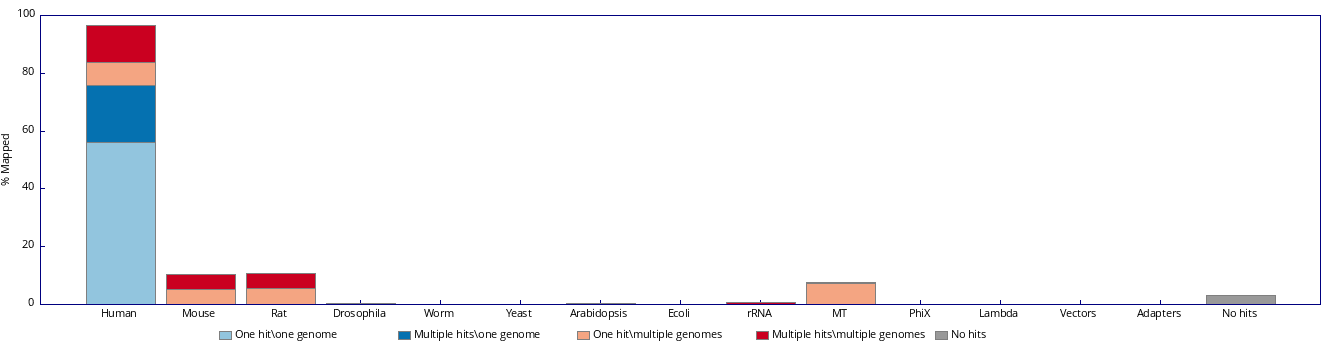
\includegraphics[width=1\textwidth]{fastqscreen_example}
    \caption[FastQScreen plot example]{An example of a good FastQScreen output result, with human mapping close to 100\% and some multi-mapping to mouse and rat genomes. } 
    \label{fig:fastqscreen_example}
\end{figure}

\subsubsection{MultiQC}

\begin{itemize}\itemsep-0.5em
\item[] \textbf{Citation}: 				\cite{multiqc}
\item[] \textbf{Documentation}: 	\url{https://multiqc.info/docs/}
\item[] \textbf{Dependencies}:  Python 3
\end{itemize}

MultiQC provides a convenient way of collating multiple QC reports across multiple samples into a single interactive HTML report. It supports the input of 114 tools as of version 1.11, including the reports from tools found further downstream, in the preprocessing, alignment or quantification parts of the pipeline. 

\subsection{Preprocessing}
If poor quality data is identified, it should be cleaned to avoid negative effects in the downstream analysis. Quality trimming which is too aggressive may similarly negatively impact downstream analysis, thus care must be taken to select appropriate quality thresholds \citep{davis2019}. Some \citep{liao2020read} doubt the necessity of trimming at all.

\subsubsection{Cutadapt: Short reads and Adapter sequences}
\label{cutadapt}
\begin{itemize}\itemsep-0.5em
\item[]\textbf{Cutadapt citation}: 				\cite{martin2011cutadapt}
\item[]\textbf{Cutadapt documentation}: 	\url{https://cutadapt.readthedocs.io/en/v4.0/guide.html}
\item[]\textbf{Cutadapt dependencies}: Python 3.7 or newer
\item[]\textbf{Trim Galore! citation}: 				\cite{trimgalore}
\item[]\textbf{Trim Galore! documentation}: 	\url{https://www.bioinformatics.babraham.ac.uk/projects/trim_galore/}
\item[]\textbf{Trim Galore! dependencies}: cutadapt, FastQC
\end{itemize}


One of the primary functions of Cutadapt (as indicated by its name) is to trim adapter sequences, which may be given as a string following the \texttt{-a} parameter. Additionally, Cutadapt may be given a read length threshold (\texttt{--length}) to remove short reads which are susceptible to multimapping and ambiguity during alignment \citep{deschamps2020handling}. 

Trim Galore! is a wrapper script that may be used to instantly redirect the trimmed reads from Cutadapt back to FastQC to reassess the data quality. It accepts the same arguments as Cutadapt, with an additional \texttt{--fastqc\textunderscore args} which accepts additional arguments to be passed on to FastQC as a string. This combines both Cutadapt and FastQC parameters into a single command. 

\begin{itemize}\itemsep0em
\item[] \textbf{Cutadapt's default options:}
\item Outputs the trimmed FASTQ file and simultaneously generates its FastQC report.
\item Assumes Sanger/Illumina 1.9 quality encoding (ASCII code +33 = Phred score)
\item Trims adapter and up- or downstream sequence
\item Allows a maximum error rate of 10 \% (Error rate = number of errors divided by length of matching region)
\item Removes up to one adapter per read
\item Requires a three nucleotide overlap between read and adapter for an adapter to be found
\end{itemize}


\subsubsection{Prinseq++: Low complexity and No Basecalls}
\begin{itemize}\itemsep-0.5em
\item[] \textbf{Short for}: 				PReprocessing and INformation of SEQuence data
\item[] \textbf{Citation}: 				\cite{prinseq++}
\item[] \textbf{Documentation}: 	\url{https://github.com/Adrian-Cantu/PRINSEQ-plus-plus}
\item[] \textbf{Dependencies}: C++
\end{itemize}
% Useful http://prinseq.sourceforge.net/manual.html
Ambiguity in reads may manifest itself in the form of low complexity regions, and reads with a high number of \textit{N}'s, in addition to those discussed in Section \ref{cutadapt}. The data should be filtered to some degree based on these metrics, which is facilitated by ready-made tools such as Prinseq++. Prinseq++ is a C++ multi-threaded implementation of the perl-coded Prinseq-lite software \citep{schmieder2011quality}. 

Regions of low-complexity (also called compositionally biased regions) are a natural part of biological sequences, playing an important role in protein translation \citep{frugier2010low}, and have a functional role in some proteins \citep{ntountoumi2019low}. Nevertheless, due to their repetitive nature, they tend to result in multimapping and low alignment confidence scores, especially when exacerbated with short read lengths. To quantify low-complexity regions, Prinseq++ present the DUST (Tatusov and Lipman, unpublished) and Entropy approaches. Both are different algorithms which employ a scoring function based on nucleotide frequencies which ultimately generate a score between 0 and 1 as a measure for sequence complexity  \citep{morgulis2006fast}. The DUST module is incorporated in BLAST \citep{altschul1997gapped} for the same purpose, to mask low-complexity regions. Prinseq++ filters reads which exceed the stipulated DUST score (\texttt{-lc\textunderscore dust}) or Entropy (\texttt{-lc\textunderscore entropy}) thresholds.

The ambiguous base \textit{N} represents no basecall, and a threshold for the maximum number of \textit{N}'s in a sequence may be set using \texttt{-ns\textunderscore max\textunderscore n}.
    
\begin{itemize}\itemsep0em
\item[]\textbf{Prinseq++'s default options:}
\item Outputs the filtered FASTQ, and the filtered reads as separate files.
\item Removes sequences with a DUST score < 0.5
\item Removes sequences with an Entropy score < 0.5 
\item Trims recursively from both ends of the sequence chunks of length 2 if the mean quality of the first 5 bases is <20 
\end{itemize}

\subsection{Alignment}

Quick and computationally efficient pairwise comparison and alignment of two sequences consisting of billions of reads is a classic problem in bioinformatics. We have amassed large volumes of literature describing potential strategies to tackle the problem, occupying different niches.

Aligners may take one of two approaches: global alignment or local alignment. Global alignment algorithms, such as \cite{needleman1970general}, aligns both sequences from their first amino acid residue through to their last and is more suitable for sequences of approximately equal lengths. By contrast, local alignment algorithms, such as \cite{smith1981identification} and BLAST, are more suited for sequences that are suspected to overlap only partially. 

There are some semantics associated with this particular step which should be clarified before proceeding further. \textit{Alignment} and \textit{mapping} are often used interchangeably, but there are subtle differences. According to the BioStar Handbook \citep{albert2020biostar}, which cites a presentation by Heng Li, \textit{alignment} is the optimal placement of a read against a genome, while \textit{mapping} suggests less certainty, and that the optimal placement is not always possible. Which term to use is dependent on the algorithm, although modern tools often combine the two approaches, which continues to blur the line separating the terms \citep{albert2020biostar}.

In RNA-seq, the reference sequence one aligns against may be either a genome or a transcriptome. Since reads from our FASTQ file originate from processed mRNA, the reads may span across multiple exons. This cannot be simply mapped onto a reference genome because of the presence of intronic and non-coding regions \citep{rnadataanalysis2020}. To map transcript-derived reads which against a genome, a splice-aware aligner must be used (\autoref{fig:alignment}).

\begin{figure}[!h]
    \centering
    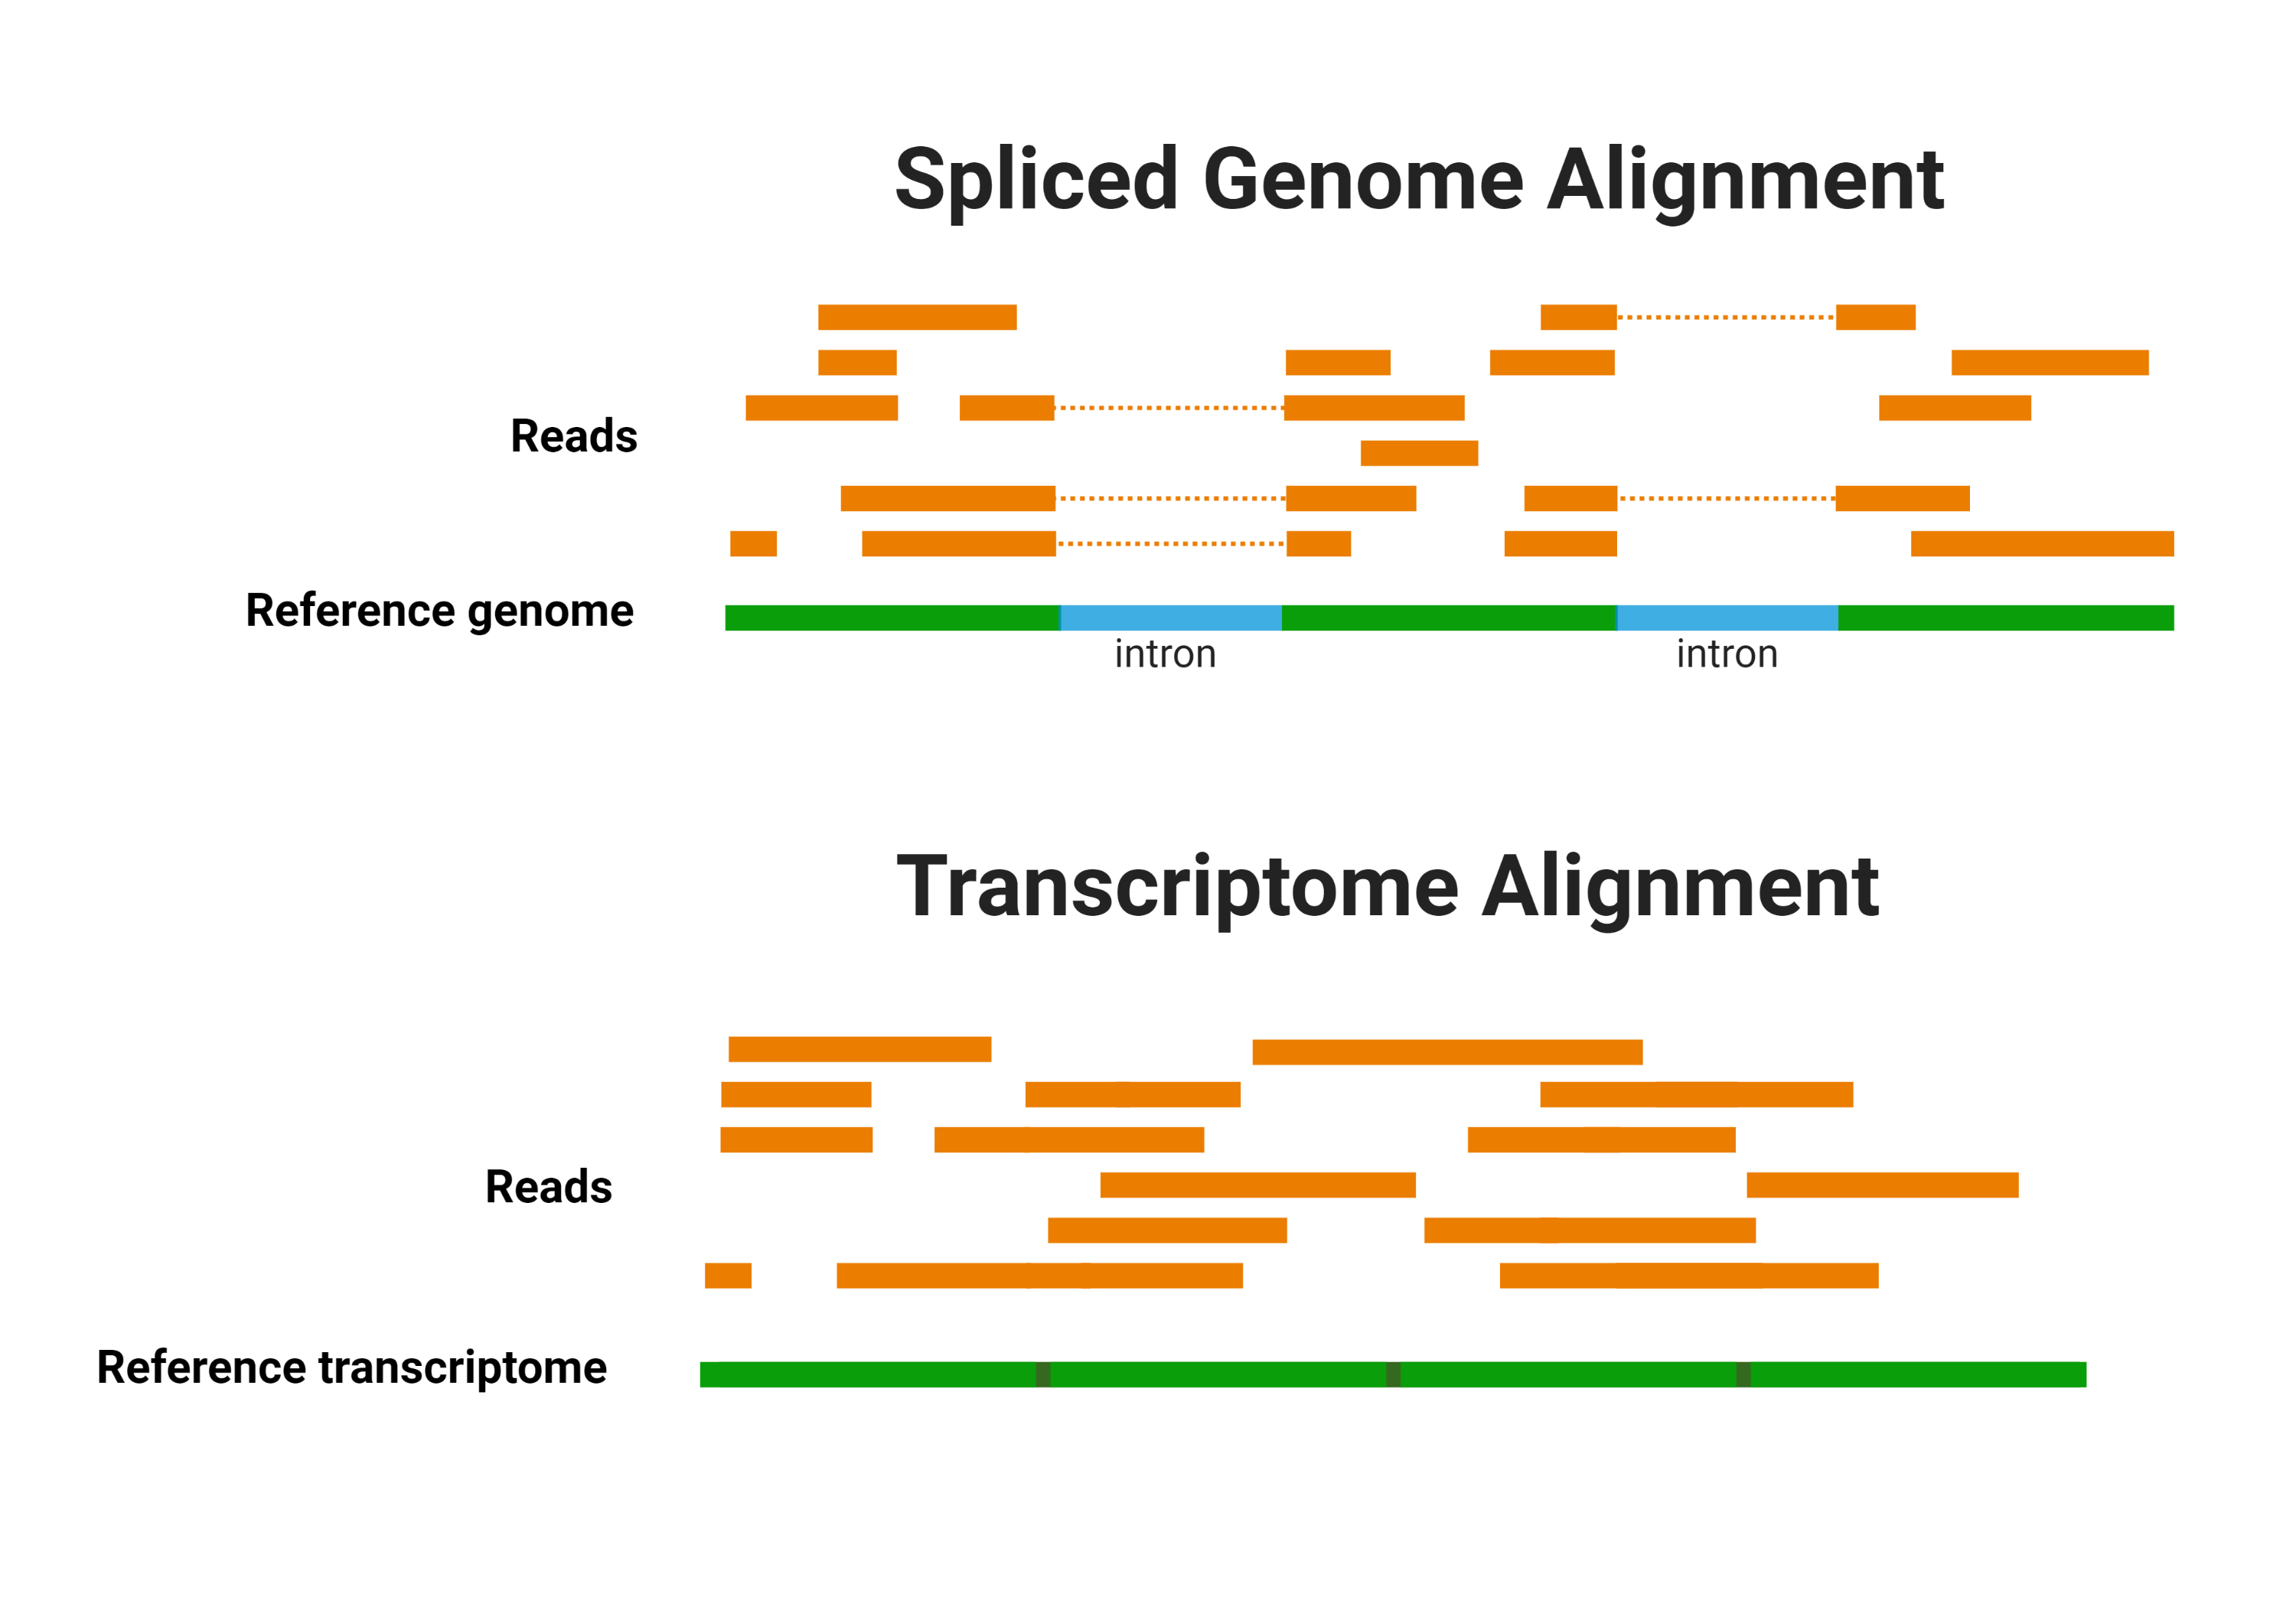
\includegraphics[width=13cm]{transcriptome_vs_genome_alignment}
    \caption[Alignment against a reference genome or a reference transcriptome]{Alignment against a reference genome or a reference transcriptome. Created using \href{https://biorender.com/}{BioRender.com}. } 
    \label{fig:alignment}
\end{figure}
%%\clearpage

Alignment algorithm efficiency is at least semi-dependent on read length, with each having ideal range of lengths, although this is rarely stated in the documentation \citep{albert2020biostar}. A distinction is often made between short-read and long-read mappers, although this distinction is arbitrary. Many conventional short-read mappers are not suitable for reads under 30bp, necessary for the study of small RNAs \citep{albert2020biostar, ziemann2016evaluation}.

Quasi-mappers and pseudo-aligners (most notably Salmon \citep{patro2017salmon} and Kallisto \citep{bray2016near} respectively) differ from classical alignment. They utilise \textit{k}-mer matching to match reads and corresponding transcripts \citep{rnadataanalysis2020}. They require less runtime than other existing alignment tools \citep{Zhang2017}, while their accuracy is disputed, with \cite{srivastava2020alignment} finding that they are less accurate and \cite{Zhang2017, Schaarschmidt2020} argue that their accuracy is comparable to conventional aligners.

Some implementation of the mapping quality (MAPQ) value is used by all conventional aligners and it is a standard field in the SAM/BAM file formats. It is analogous to the Phred score in a FASTQ file, and allows for easy filtering of bad quality reads. Unlike the Phred score, there is no single standardised definition or formula, with slight variations existing across various sources \citep{andrews2016mapq}.

%\subsubsection{The Reference Genome}

\subsubsection{STAR}
\begin{itemize}\itemsep-0.5em
\item[] \textbf{Short for}: 				Spliced Transcripts Alignment to a Reference
\item[] \textbf{Citation}: 				\cite{Dobin2013}
\item[] \textbf{Documentation}: 	\url{https://physiology.med.cornell.edu/faculty/skrabanek/lab/angsd/lecture_notes/STARmanual.pdf}
\item[] \textbf{Dependencies}: 64 bit Linux or Mac OS X
\end{itemize}

STAR is an open-source software package that performs local, splice-aware alignment in two major steps: (1) seed search and (2) clustering, stitching and scoring. It was coded in C++ for the specific purpose of mapping RNA-seq reads to a genome.
%It requires a considerable amount of RAM to run efficiently \citep{•}, and requires more runtime than Quasi-mappers and pseudo-aligners
% Suffix arrays

The algorithm first searches for the Maximum Mappable Prefix (MMP) which acts a seed from which to extend its alignment. This must be an exact identical match with the reference genome. These MMPs are clustered according to proximity to identify a set of \textit{anchor} seeds. STAR stitches together the seeds identified in the first step, and if alignment within one window does not cover the entire read, it will try to find multiple windows to cover the read, resulting in a chimeric alignment. This means that different parts of the same read may map to distant genomic loci, possibly to different strands or chromosomes, which is especially useful when dealing with cancer-derived transcriptomes given the frequency of structural variants. A local alignment scoring system guides the stitching, with matches, mismatches, indels and splice junction gaps translating to different scores.
%Perhaps a diagram here

An index must be generated prior to alignment, which is generated from a reference genome and its respective annotation file in the GTF format. This hastens the algorithm in a way similar to how one might use the index in a book, which points to the specific locations of certain headers \citep{trapnell2009map}.

STAR provides the user with great flexibility, with many parameters, such as  the scoring system weighting and the size of search windows, being user-defined. \cite{dobin2015mapping} provide excellent descriptions of nine different datatype- and output-dependent strategies that one may take when mapping RNA-seq reads with STAR. 

% perfect paper: https://currentprotocols.onlinelibrary.wiley.com/doi/abs/10.1002/0471250953.bi1114s51 
% sci hub for it: https://sci-hub.hkvisa.net/10.1002/0471250953.bi1114s51

\begin{itemize}\itemsep0em
\item[] \textbf{STAR's default options:}
\item Generates a genome index using a reference file and its respective annotation (GTF) file.
\item Aligns an experimental transcriptome using the genome index and outputs an alignment file (SAM, unsorted BAM or BAM sorted by coordinates) and various log files.
\item Uses a mapping quality metric MAPQ, calculated as $10*log_{10}(1-\frac{1}{N_{map}})$, where ${N_{map}}$ is the number of places the read maps to. A value of 255 is given to uniquely mapped reads.
\item Passes on \texttt{NH HI AS nM} as SAM attributes as defined in the SAM format specifications \footnote{\url{https://samtools.github.io/hts-specs/SAMv1.pdf}}.
\end{itemize}

%Multimapping:https://www.sciencedirect.com/science/article/pii/S2001037020303032

\subsection{Quantification}
\label{quantification}
% Detailed paper: https://arxiv.org/pdf/1104.3889v2.pdf
The following step associates the aligned reads with the respective genes or transcripts found at their locus. The counts of the mapped reads are proportional to the cell's expression of that particular gene/transcript. Quantifying at the transcript-level is more detailed than the gene-level, but not all research questions require this level of detail. The final output of the combined samples should be a table resembling \autoref{tab:read_count}.

\cite{pachter2011models} provides a detailed (albeit slightly outdated) review of the mathematical models behind transcript quantification, such as the Expectation–Maximization (EM) algorithm, and how they affect downstream analyses. EM estimates the maximum likelihood of proper alignment in the presence of latent variables \citep{brownlee2019gentle, pachter2011models}.

\begin{table}[h]
\centering
\caption{An example of a read count table, values representing the number of reads aligned to that gene. In bulk RNA-seq, each sample represents the pooled RNA of a large number of cells, most likely of different cell types.}
\label{tab:read_count}
\begin{tabular}{lllll}
\textbf{Genes} & \textbf{Sample$_{1}$} & \textbf{Sample$_{2}$} & \textbf{Sample$_{3}$} & ...  \\
A2BG  & 10      & 30      & 0       & ...  \\
AML   & 30      & 3       & 3       & ...  \\
AMT2  & 0       & 0       & 10      & ...  \\
ARST5 & 5300    & 1900    & 3250    & ...  \\
...   & ...     & ...     & ...     & ... 
\end{tabular}
\end{table}

\subsubsection{RSEM}
\begin{itemize}\itemsep-0.5em
\item[] \textbf{Short for}: RNA-Seq by Expectation Maximization
\item[] \textbf{Citation}: 				\cite{li2011rsem}
\item[] \textbf{Documentation}: 	\url{http://deweylab.github.io/RSEM/README.html}
\item[] \textbf{Dependencies}: 64 bit Linux/Mac OS, C++, Perl, R, STAR/HISAT2/Bowtie2
\end{itemize}

RSEM uses a statistical model based on \cite{li2010rna}, an implementation of the EM algorithm to address the issue of ambiguous read mapping, and assign reads to their appropriate gene or transcript. RSEM gives the user the option to produce both, and normalises the counts in the process. For each sample, RSEM produces two tab-delimited text files: one quantified at the gene-level and another at the transcript-level. Each row of these file represents the respective gene or transcript (the transcript file is larger due to alternative splicing), with the columns including the IDs, expected counts and normalised counts (TPM and FPKM)

An aligner (STAR, Bowtie2 or HISAT2) may be called directly through RSEM, to combine alignment and quantification (and potentially normalisation) into a single step. The genome index to be used by the aligner may be generated through \texttt{rsem-prepare-reference} and alignment + quantification may be performed with \texttt{rsem-calculate-expression}.

\begin{itemize}\itemsep0em
\item[] \textbf{RSEM's default options:}
\item Accepts FASTQ files as input for alignment.
\item Outputs a gene-centric file, with the following columns: \texttt{gene\textunderscore id, transcript\textunderscore id(s), length, effective\textunderscore length, expected\textunderscore count, TPM and FPKM}
\item Outputs a transcript-centric file, with the following columns: \texttt{transcript\textunderscore id, gene\textunderscore id, length, effective\textunderscore length, expected\textunderscore count, TPM, FPKM, IsoPct}
\end{itemize}

\subsection{Normalisation}

To adjust for confounding variables which are not biologically relevant, the read counts must first be normalised. The main factors to account for are sequencing depth \citep{robinson2010scaling}, gene length \citep{oshlack2009transcript} and GC content \citep{risso2011gc}. Effective gene expression analysis should calculate the abundance of the transcripts as a fraction of the entire RNA repertoire for that particular sample. A number of methods have evolved over the years to tackle these issues. \cite{dillies2013comprehensive} and \cite{bullard2010evaluation} extensively explore the different approaches one may take. Despite their frequent misuse in published studies, within-sample comparison methods (FPKM \citep{trapnell2010transcript}, RPKM \citep{mortazavi2008mapping}, TPM \citep{li2011rsem}, Total Counts \citep{dillies2013comprehensive}) should be avoided in \ac{DGE} analysis as they only account for differences within the same sample, and not between samples \citep{dundar2015introduction, zhao2020misuse}.

\begin{figure}[!h]
    \centering
    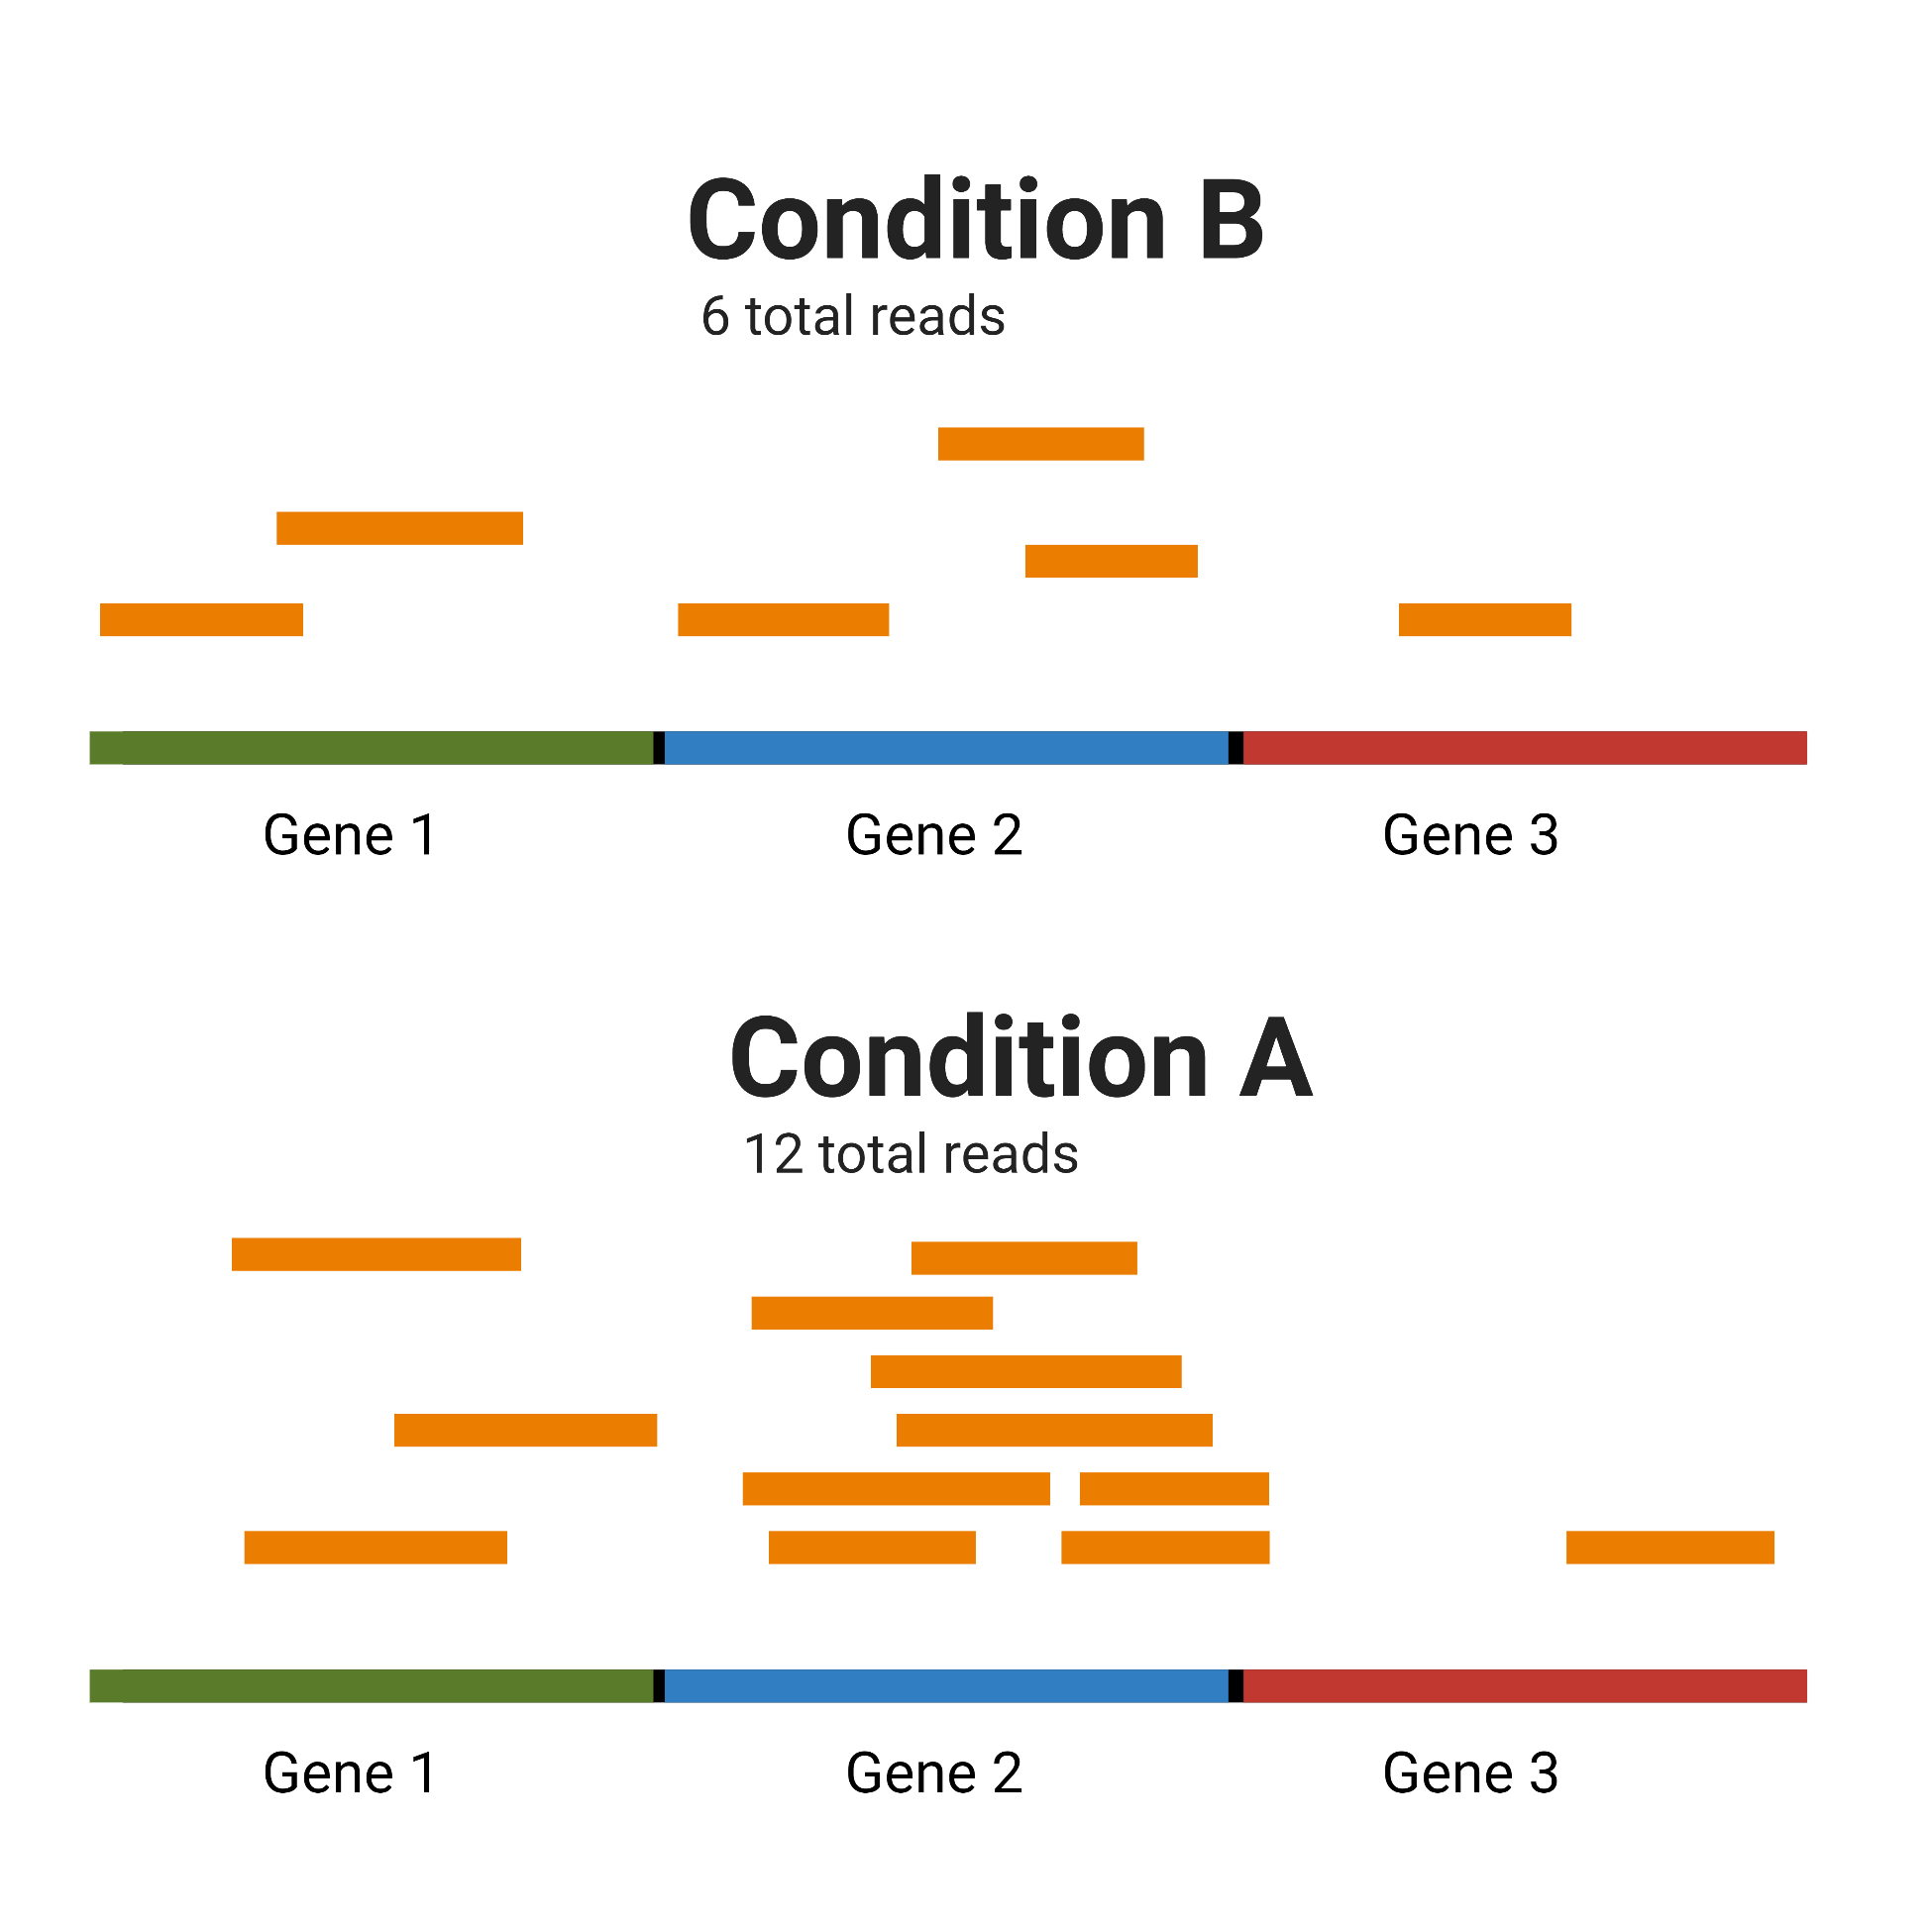
\includegraphics[width=9cm]{library_differences}
    \caption[Differences in library composition between samples]{Potential differences between samples in library composition. Condition A has more reads aligned to Gene 1 than Condition B, but it is considered more highly expressed in Condition B since the \textit{proportion} of the reads is higher. After accounting for library differences, Gene 2 is more highly expressed in Condition A, and Gene 3 is more highly expressed in Condition B. Created using \href{https://biorender.com/}{BioRender.com}. } 
    \label{fig:lib_diff}
\end{figure}
%%\clearpage

\subsubsection{Trimmed Mean of \textit{M}-values (TMM)}
\label{TMM}

The \ac{TMM} is implemented in edgeR \citep{edger} through the \texttt{calcNormFactors} function. It is recommend by the edgeR vignette\footnote{\url{https://www.bioconductor.org/packages/release/bioc/vignettes/edgeR/inst/doc/edgeRUsersGuide.pdf}} if one wishes to continue performing \ac{DGE} analysis using that library. It was first introduced in \cite{robinson2010scaling}, who explain the underlying mathematics in detail. \ac{TMM} assumes that the majority of genes, in both samples, are not differentially expressed, although the model is robust against deviations to this assumption \citep{robinson2010scaling}. 

\ac{TMM} performs better for between-samples comparisons, as opposed to within-sample comparisons \citep{dundar2015introduction}. \cite{robinson2010scaling} recognise that it makes intuitive sense that differences in library size should be normalised (i.e. depth or coverage, as seen in \autoref{fig:lib_diff}), but they consider this scaling too simplistic for many biological applications. 

The observed counts for gene \textit{g} in library \textit{k}, calculated from the read quantification step (\autoref{quantification}), are represented as $Y_{gk}$. The total reads in library \textit{k} are represented as $N_k$. The  \textit{M}-value for gene \textit{g} and libraries \textit{k} and \textit{k'} may be calculated as:

$$ M_g = log_2 \frac{Y_{gk}/N_k}{Y_{gk'}/N_{k'}}$$

The absolute expression level, \textit{A}, for gene \textit{g} is calculated as:

$$A_g = \frac{log_2(Y_{gk}/N_k)*Y_{gk'}/N_{k'}}{2}$$

The next step is to trim the means of the \textit{M}-values and \textit{A}-values. A mean is trimmed when a percentage of the data is truncated at the upper and lower ends. By default this is 30\% for the \textit{M}-values and 5\% for the \textit{A}-values, but these settings may be changed \citep{robinson2010scaling}. 

The final step is the calculation of the normalisation factor and weighted mean of the trimmed $M_g$ using precision (inverse of the variance) weights. The calculations used in this step are too complex for the scope of this project (see \cite{robinson2010scaling} for further details). 


\subsection{Differential Expression Analysis}
% rlly good for DGE file:///C:/Users/matth/OneDrive/Desktop/Msc%20Bioinformatics/!MMB5010%20DISSERTATION-DESKTOP-A2009SI/Literature/Tutorials/Introduction%20to%20differential%20gene%20expression%20analysis%20using%20RNA-seq.pdf 
The crux of the RNA-seq pipeline is to decide through statistical testing whether a given gene's expression varies significantly between samples, and if this variation can be explained by the difference in the cells' biology. Genes with very low read counts cannot be reliably represented across all samples, and are indistinguishable from background noise \citep{mcintyre2011rna}. These lowly expressed genes should be filtered before differential expression analysis as they are more likely to be incorrectly identified as \ac{DEG}s. All tools which measure gene expression aim to estimate two metrics  based on normalised read counts from replicated samples: 

\begin{enumerate}\itemsep-0.5em
\item The \textit{magnitude} of the differential expression, represented as the \ac{logFC}.
\item The \textit{significance} of the difference, represented as a \textit{p}-value adjusted for multiple testing.
\end{enumerate} 

The three most commonly used tools for \ac{DGE} judging by citation counts at the time of writing are DESeq2 \citep{love2014moderated}, edgeR \citep{edger} and limma \citep{ritchie2015limma}, which all take the same basic approach. Regression-based models are used to estimate the difference in normalised read counts for each gene or transcript of interest, which are tested for a significant difference \citep{dundar2015introduction}.

In differential expression analysis we are testing whether each gene in our list is significantly up- or down-regulated when compared to the reference sample. This test is performed for thousands of genes, which is where we run into the multiple testing problem. These large numbers of comparisons suddenly make small Type I error rates relevant, running the risk of falsely identifying certain genes as differentially expressed. To account for this risk, \textit{p}-values are adjusted based on how many tests are to be considered \citep{feise2002multiple}. The Bonferroni correction \citep{dunn1961multiple} is one such method, although considered by some \citep{feise2002multiple} to be too conservative, potentially tipping the scale to the other end and inducing Type II errors (declaring a result not statistically significant when it is). Other, less conservative solutions have been proposed, such as the Bonferroni-Holm \citep{holm1979simple} or Hochberg \citep{hochberg1987multiple} techniques.

%Very low read counts cannot be reliably distinguished from background noise so these need to be filtered: https://pubmed.ncbi.nlm.nih.gov/21645359/
\subsubsection{EdgeR}
\label{EdgeR}

The Bioconductor package edgeR allows the implementation of a wide array of statistical methods applicable to \ac{DGE} analysis. EdgeR accepts a matrix of reads normalised by \ac{TMM} as input (see Section \ref{TMM} for details). Prior to differential expression analysis, this matrix is filtered according to read counts using the function \texttt{filterByExpr} which removes genes with <10 read counts. Two primary routes may be taken using \autoref{fig:edger_options}, the classic route which involves exact tests \citep{robinson2007moderated, robinson2008small}, or the Generalized Linear Model (GLM) route, although certain features of the two may be combined. The GLM tests for \ac{DGE} are likelihood ratio tests (LRTs) \citep{mccarthy2012differential} and quasi-likelihood F-tests (QLFs) \citep{lun2016s, lund2012detecting}.

The \texttt{exactTest} function is based on quantile-adjusted conditional maximum likelihood (qCML) method. It produces a matrix of pseudo-counts\footnote{Note that the meaning of the term \textit{pseudo-counts} may change according to the context, and may be used by other studies to refer to something different.} which are designed to speed up computational analysis and not to be interpreted as regular normalised counts. The qCML method is only applicable on datasets with a single factor. The exact test for a negative binomial distribution should not be confused with Fisher’s exact test \citep{upton1992fisher}, although the two share many similarities.

GLMs are an adaptation of classical linear models to cater for non-normally distributed data \citep{dunn2018generalized}. The QLF dispersion estimate and test can be performed with the functions \textit{glmQLFit} and \textit{glmQLFTest}. This fits a negative binomial GLM to the \ac{TMM} normalised read counts. The LRT compares the goodness of fit of two competing models through the functions \textit{glmFit} and \textit{glmLRT}.

\begin{figure}[h!]
    \centering
    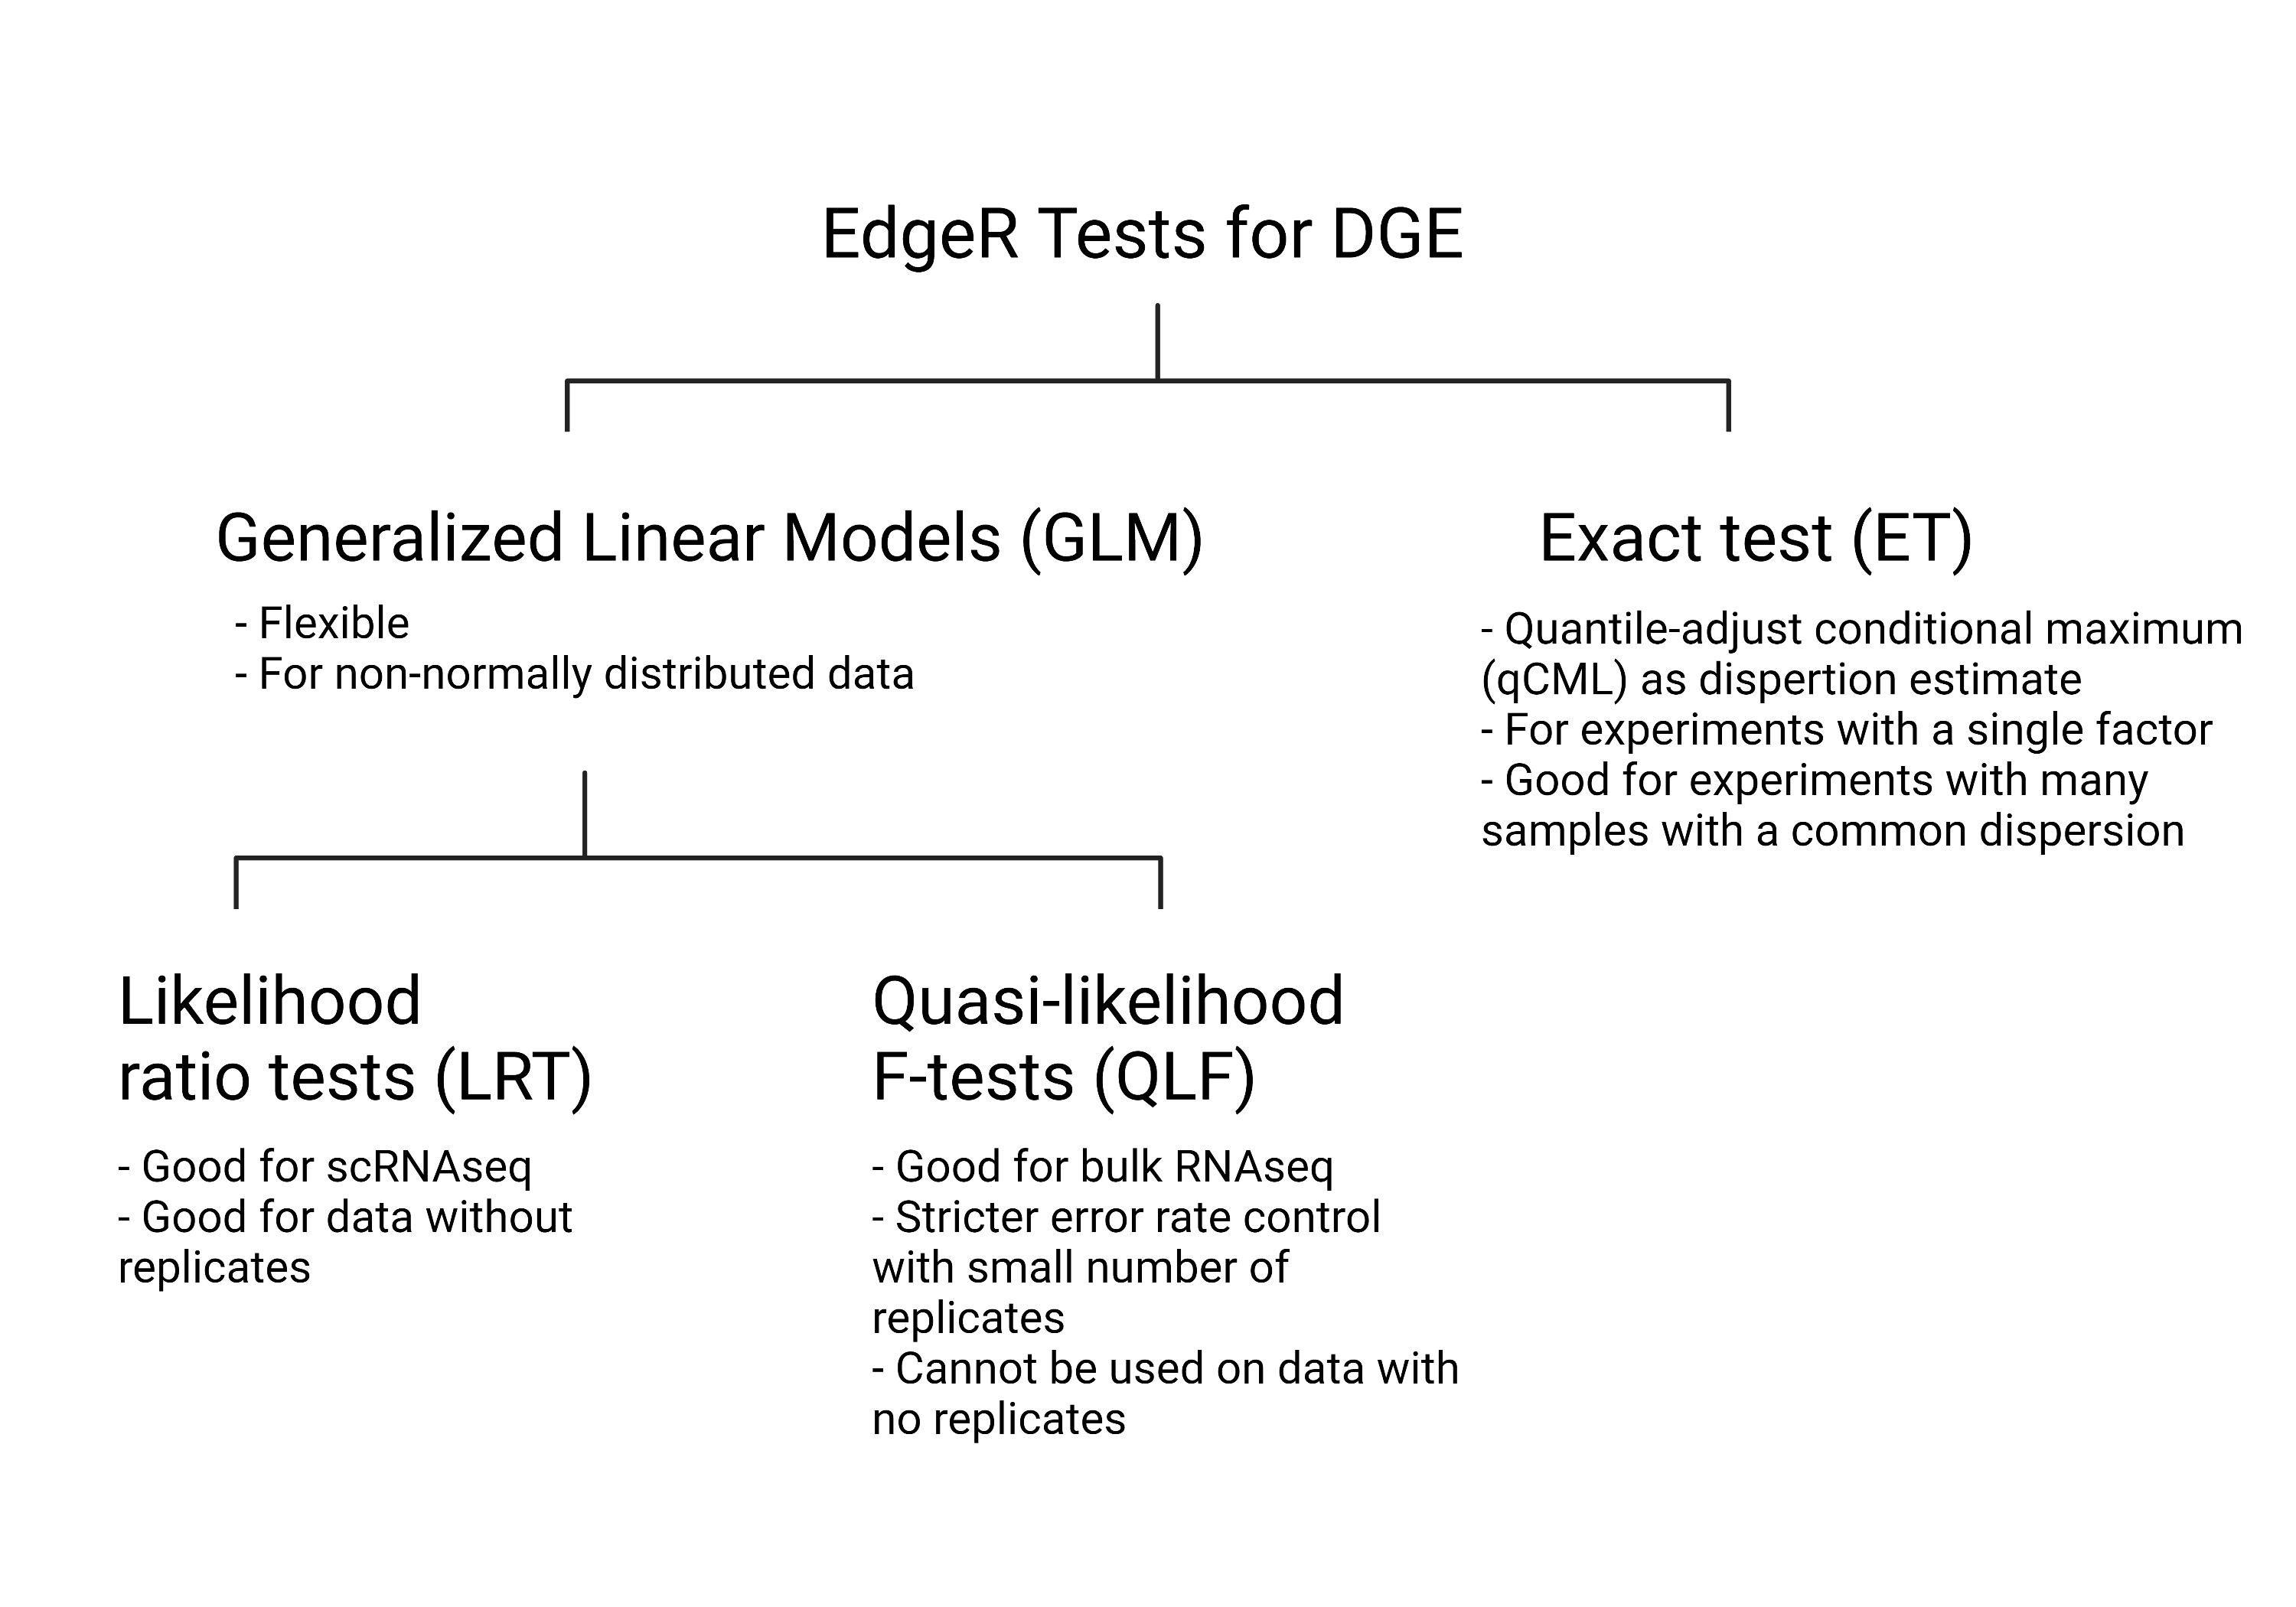
\includegraphics[width=13cm]{edger_dge_options}
    \caption[Summary of the options provided by edgeR for DGE identification]{Summary of the three options provided by edgeR for \ac{DGE} identification, based on comments and recommendations by its vignette. } 
    \label{fig:edger_options}
\end{figure}
%\clearpage

EdgeR and DESeq2 are quite similar in that they both make use of a negative binomial distribution to model read counts, and estimate dispersion based on the approximate conditional inference, first proposed by \cite{cox1987parameter}.  EdgeR is recommended for experiments with fewer than 12 replicates \citep{schurch2015evaluation}, and unlike DESeq2, allows for the analysis of data with no replicates, although highly discouraged by the vignette. 
% The negative binomial is a more general form of the Poisson distribution... maybe write some shit on this

The biggest challenge when working with data without replicates is the estimation of dispersion, which is mathematically impossible given a single sample. In cases when there is no other alternative, the vignette suggests giving a nominal value to the \ac{BCV}, from which we may derive the dispersion. The vignette suggests a few estimates for the \ac{BCV} which are based on previous experiments as the dispersion, such as \textit{0.1 for data on genetically identical model organisms}. The dispersion is equal to this value squared, which although inaccurate, is a better alternative to assuming no variance.

To account for the previously described multiple testing problem, the \texttt{topTags} function adjusts \textit{p}-values using the Benjamini-Hochberg method \citep{benjamini1995controlling} to control the \ac{FDR}. This produced value is the proportion of false positives one might expect to get from a test. 

To gain further biological insight, the \texttt{goana} and \texttt{kegga} functions may be used to annotate genes according to their associated \ac{GO} terms and \ac{KEGG} pathways respectively. This may be particularly useful in downstream tests for gene set analyses.

The end result should be an edgeR object containing a matrix of each the \ac{logFC}, adjusted \textit{p}-values and (optionally) annotations for each differentially expressed gene. The final step is filtering on the matrix by setting a (largely arbitrary) \ac{logFC} and/or \textit{p}-value cutoff, and sorting the data by one of these metrics for easier biological analysis.
% Visit later and suggest values

\subsection{Downstream Analysis}
% alternative splicing, functional analysis, gene fusion detection and eQTL mapping
The steps of the pipeline up until this point are quite standard, although there are various approaches one may take, the aim of each step is clear and consistent across all RNA-seq studies. Further exploration of the data is highly specific to the experimental design and research question. Putting the data into its biological context is a type of sanity check. Deviation from biological expectations is often an indication of issues in the upstream analysis.

\subsubsection{Graphical Representation}

Graphical representation of the gathered information about the samples thus far conveys the information in a more human-readable format and allows for easier pinpointing of differences and potential batch effects. In plots which cluster data according to similarity, replicates should form distinct clusters. Two replicates which apparently switched clusters is a good indication of a potential sample swap. 

%Sashimi plot
\begin{enumerate}
\item[] \textbf{Multidimensional Scaling (MDS)} \hspace{0.15cm} RNA-seq data deals with thousands of dimensions, making it difficult to interpret and impossible to use conventional plotting methods. MDS is type of non-linear dimensionality reduction used to mitigate this issue \citep{yin2007nonlinear}. It is a between-sample measure of similarity which plots pairwise distances using Cartesian coordinates \citep{mead1992review}. 

\item[] \textbf{Principal Component Analysis (PCA)} \hspace{0.15cm} Similar to MDS in scope except that it is a \textit{linear} dimensionality reduction technique. PCA transforms the data to find the combination of variables which explains the maximum variation in the data. 

\item[] \textbf{Heatmaps and Clustering} \hspace{0.15cm} Often used in combination with each other, with a colour gradient in the heatmap signifying the  logFC for each \ac{DEG} in the list, which are clustered according to similar expression patterns.

\item[] \textbf{Mean-Difference (MD)} \hspace{0.15cm} In other fields, it is used to determine if two methods of measurement are in agreement \citep{fry2008visualizing}. In RNA-seq it is used to compare the \ac{logFC} of each gene of a given sample against the mean \ac{logFC} of that respective gene.

\item[] \textbf{Volcano Plot} \hspace{0.15cm} Plots the results of differential expression that plots the significance (adjusted \textit{p}-values) against the \ac{logFC}. Thresholds of each are often indicated by a change in colour of the points.
\end{enumerate} 

%Include some examples?

\subsubsection{Annotation and Enrichment Analyses}

The differentially expressed gene matrix may be annotated using the AnnotationDbi \citep{annotationdbi} R package which may access annotation libraries such as the human org.Hs.eg.db \citep{org.Hs.eg.db} which is based on Entrez gene identifiers \citep{maglott2005entrez}. The systems biology of the data is of particular interest to this project, which may be investigated with enrichment analyses. % or STRING \citep{szklarczyk2016string}
\ac{GO} terms and \ac{KEGG} \citep{kanehisa2017kegg} pathway enrichment allow for comparisons between genes according to their functional role in a biological system. Further enrichment analyses may fork into three approaches, as described by \citep{khatri2012ten} and \cite{alhamdoosh2017combining}:

\begin{enumerate}
\item[] \textbf{Over-Representation Analysis (ORA)} \hspace{0.15cm} The gene list emerging from differential expression is compared to a list of genes associated with a specific pathway. The genes which overlap between the input list and the pathway list are tested for over- or under-representation (usually based on hypergeometric, chi-square, or binomial distribution) \citep{khatri2012ten}. While this information is useful, ORA is limited in that it only tests for the presence of a gene, and ignores any additional information (\ac{logFC}s, \textit{p}-values, the effect of its products on other genes, etc).

\item[] \textbf{\ac{GSEA}} \hspace{0.15cm} The limitations to the ORA approach led to the development of an alternative method, GSEA. The philosophy behind GSEA is that although large fold-changes in individual genes can have a significant biological effect, so can weaker changes in genes with a disproportionate effect on the pathway. \cite{luo2009gage} describe the term \textit{gene set} as a pre-defined group of functionally related genes, which may share a common biological pathway or ontology term. \ac{GSEA} is generally performed in three steps: (i) generation of gene-level statistics (e.g. ANOVA) which may be transformed (e.g. absolute values), (ii) statistical results are combined into a single value per gene set (e.g. Wilcoxon rank sum \citep{barry2005significance}) and (iii) the statistical significance of the gene-set-level statistic are assessed. Although an improvement over the previous method, GSEA treats gene sets separately and does not consider that a gene may be involved in multiple sets.

\item[] \textbf{Pathway Topology (PT)} \hspace{0.15cm} Building upon the previous two technologies, PT approaches take into account interactions between gene products, and the nature of their interaction (e.g. activation or inhibition). KEGG and STRING \citep{szklarczyk2019string} are examples of knowledge-bases which have sufficient information to perform PT. There are several potential approaches which are difficult to generalise but are reviewed extensively in \cite{ihnatova2018critical} and \cite{ma2019comparative}.

\end{enumerate} 

\subsubsection{GAGE and Pathview}
%Put header here like other tools?
%Generally Applicable Gene-set Enrichment (GAGE).
% https://bioconductor.org/packages/release/bioc/vignettes/gage/inst/doc/RNA-seqWorkflow.pdf
GAGE \citep{luo2009gage} performs \ac{GSEA}, where gene-set-level statistics are generated to check which gene sets are differentially expressed. %revsit 
GAGE performs pair-wise comparison between samples by default to test for significantly differentiated KEGG pathways. 

Pathview \citep{luo2013pathview}, like GAGE, is a Bioconductor \citep{gentleman2004bioconductor} R package which visualises GAGE results as an image of the chosen KEGG pathway highlighting the differentially expressed genes according to their \ac{logFC}s. Its sister library SBGNview \citep{dong2022sbgnview} offers a wider array of gene set knowledge-bases such as PANTHER \citep{mi2005panther}, Reactome \citep{croft2010reactome} and SMPDB \citep{frolkis2010smpdb}. Pathview supports two methods for pathway visualisation: the native KEGG view and the third party Graphviz \citep{ellson2001graphviz}. \cite{luo2013pathview} states that Graphiz provides better control over the graphical nodes and edges, at the expense of certain pathway metadata, namely cell types and temporal information.

\ac{GO} term analysis is supported by GAGE, although frequently neglected due to the popularity of \textit{pathway} analysis as opposed to the more generalised \textit{gene set} analysis \citep{luo2009gage}. Since \ac{GO} terms do not contain information on molecular interactions, pathways similar to those constructed by Pathview are not an option. The data may be represented by heatmaps or scatterplots as arguments in the \texttt{geneData} function.

%Include pathview image?


\clearpage
\section{Evaluation Criteria}
Every step in the pipeline is followed by some form of QC and potentially filtering of bad data, from trimming adapter sequences to filtering multimapped reads to removing very lowly expressed genes. It is not unlikely that errors of any form slip through, and for these reason the final results will be evaluated.

The list of \ac{DEG}s will be checked against a list of housekeeping genes which will act similar to negative controls. Housekeeping genes are required for basic cellular function and must be expressed in both normal and pathological cells. While they may be differentially expressed in some cases \citep{greer2010housekeeping}, they are generally uniformly expressed with low variance. Repositories such as the Housekeeping and Reference Transcript Atlas (HRT Atlas) \citep{hounkpe2021hrt} were used as sources for the gene lists. % REVISIT THIS!!
The genes and pathways affected by cancer, even those specifically affected by \ac{AML} are well studied, annotated and aggregated in repositories such as GeneCards \citep{stelzer2016genecards} or OMIM \citep{hamosh2005online}. Thus the biological relevance of these genes in relation to these pathways will be checked.

In future work, if more funds are acquired, similar work could be conducted with more technical replicates to confirm the findings of this project with greater statistical power. To decrease the number of sequencing errors, Sanger Sequencing could potentially be used, given its 99.999\% accuracy rate and long read lengths of up to \textasciitilde 1000bp \citep{shendure2008next}.

\clearpage
\section{Related Work}
This multidisciplinary project is based on multiple rapidly developing fields, thus it is important for the researcher to keep updated with the latest literature. This section will describe the methods and findings of literature which this project will build upon, namely those which cover: (i) the biochemical components of extra virgin olive oil and their potential application to clinical practice, (ii) compounds with chemotherapeutic potential in \ac{AML} and the resultant \ac{DEG}s and (iii) tools to construct an effective RNA-seq pipeline given our specific data.

\subsection{Biochemistry of Olive Oil}
The Mediterranean diet is rich in fruits, vegetables, fish, and olive oil, and is linked to lower rates of atherosclerosis, cancer and cardiovascular disease \citep{owen2000, tripoli2005phenolic, cicerale2012antimicrobial, fabiani2002cancer}. This is attributed in part to the higher intake of extra virgin olive oil, and more specifically, its phenolic compounds. These have been the subject of extensive investigation as a result of their antimicrobial, antioxidant and anti-inflammatory properties \citep{cicerale2012antimicrobial, tripoli2005phenolic, bendini2007phenolic, serreli2018biological}. \cite{tripoli2005phenolic} attributes olive oil's slightly bitter and pungent taste to hydroxytyrosol and oleuropein, which both exhibited antioxidant activity.

\cite{owen2000} split the biochemical profile of olive oils into three classes: (i) simple phenols (e.g. hydroxytyrosol, tyrosol), (ii) secoiridoids (e.g. oleuropein) and (iii) the lignans (e.g. pinoresinol). All three classes have shown antioxidant properties.

\cite{gatt2021first} was the first to characterise the phenolic profiles of Maltese extra virgin olive oils. Through liquid-liquid extraction and liquid chromatography mass-spectrometry, they found that the major constituents are tyrosol, hydroxytyrosol (\autoref{fig:tyrosol_hydroxytyrosol}) and their derivatives. This is in accordance to olive oils from other sources (\citep{Angerosa1995}), although the compound concentrations may vary. These two classes of simple phenols have been the main focus of clinical research related to olive oil extracts.

\begin{figure}[!h]
    \centering
    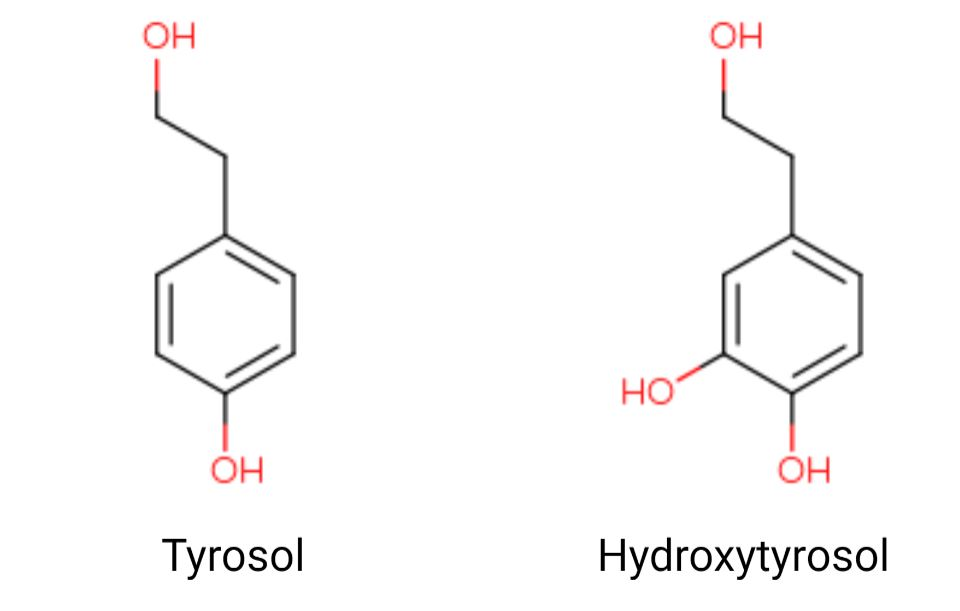
\includegraphics[width=8cm]{tyrosol_hydroxytyrosol}
    \caption[Chemical structures of tyrosol and hydroxytyrosol]{Chemical structures of tyrosol and hydroxytyrosol. The rest of the phenolic profile of extra virgin olive oils consists of derivatives of these two compounds.} 
    \label{fig:tyrosol_hydroxytyrosol}
\end{figure}


There is abundant literature on the role of natural phenolic compounds in general in the prevention and treatment of cancer. This is achieved by regulating the cell cycle \citep{jafari2014role} and the epigenome \citep{pan2015breast}. These compounds may complement traditional chemotherapeutic treatments, potentially lessening the use of chemicals with severe side-effects on the patients. \cite{gatt2021phenolic} provide a comprehensive review on phenolic effects on leukaemia \textit{in vitro}, \textit{in vivo} and in clinical practice. Literature on the effects of specifically olive oil-derived phenolic compounds on cancer shall be covered in Section \ref{Differentiation_AML}.

\subsection{Differentiation of HL-60 cells by Phenolic Compounds Derived from Olive Oil}
\label{Differentiation_AML}
There is a great medical initiative to identify compounds which induce differentiation and subsequently apoptosis in cancerous cells, and to analyse the effects these compounds have on the biochemistry of the cell. Even the seemingly specific topic of the differentiation of HL-60 cells by phenolic compounds derived from olive oil, yields myriad peer-reviewed studies, earning it a distinct section in this literature review. 

Differentiation therapy has changed the prognosis of \ac{AML}, and has shown a surge in academic interest after the success of \ac{ATRA} (see Section \ref{Treatment Methods}). In successful differentiation therapy, the undifferentiated myeloid cells will be induced to take an epigenetic path, culminating in apoptosis \citep{santos2000expression, mark2017transcriptomes}. Genes forming part of the JAK-STAT signaling pathway and the nuclear factor $\kappa\beta$ (NF-$\kappa\beta$) pathway have been repeatedly proven to play an essential role in this process, and are activated by differentiation agents \citep{matikainen1997retinoic, gianni1997stat1, cohen2005jak, ren2013resveratrol, iwata2016parp9}. Differential expression of the genes constituting  these two pathways seem to be hallmarks of successful differentiation therapy.

The similarity in experimental design and goals makes \cite{gatt2021tyrosol} a particularly relevant study to build upon and use for comparison. The study was successful in inducing differentiation and significant apoptosis in an HL-60 cell line using tyrosol derived from Maltese extra virgin olive oil as a differentiation agent. The differentiated cells exhibited morphological characteristics of neutrophils and monocytes. Three samples of cells were exposed to the phenol for three varying lengths of time (1hr, 6hr, 12hr) which were subjected to a bulk RNA-seq analysis, together with a positive monocyte differentiation control. They defined a total of 199 \ac{DEG}s. The \textit{Myeloid differentiation} \ac{GO} term (\ac{GO}:0030099) genes were significantly upregulated (OSCAR, RELB, VEGFA, GAB2, JUNB, DNASE2, ICAM, CCL3), particularly monocyte genes. Transcription factors IRF1, IRF7, STAT2, RelB, NFKB2, ATF3, and BCL3 and chemokines CCL3 and CCL4 were all found to be upregulated. At a pathway-level, Neutrophil Degranulation (CEACAM6, CLEC5A, FPR1, SERPINA1, ELANE, AZU1, PRG2) and Cholesterol biosynthesis (LSS, SQLE, ACAT2, DHCR7, HMGCS1, FDFT1) were found to be down-regulated. A complete table of \ac{DEG}s were available for download in the \textit{Supplementary Material}, which will be a useful resource for comparison.

\cite{fabiani2008inhibition} found hydroxytyrosol treatment over a period of 25 hours to bring about an upregulation in cyclin-dependent protein kinase inhibitors CDKN1A and CDKN1B, which induced apoptosis. Cell proliferation inhibition was directly proportional to the increase in time and phenolic extract concentration. The differential expression of CDKN1A coincides with the findings of \cite{gatt2021tyrosol}. \cite{fabiani2011production} confirms these findings, demonstrating that hydroxytyrosol induces apoptosis in HL-60 cells through the production of extracellular hydrogen peroxide (H$_2$O$_2$). This was not a universal property of differentiation-inducing olive oil phenolics, with some inducing apoptosis without the production of  H$_2$O$_2$ and others simply failed to induce apoptosis.

In multidrug resistant HL-60 cells, \cite{crescimanno2009effects} were able to induce apoptosis using a crude phenolic extract extracted from extra virgin olive oil of the Moraiolo cultivar. This induced the expression of monocytic CD14 cell surface antigens but not of the granulocytic CD11. The concentration of the extract was directly proportional to the percentage of apoptotic HL-60 cells. 


% The importance of VEGFA in myeloid cell differentiation has also been reported by Huang et al., 2017 while Czepluch et al., 2011 discussed its expression in two monocyte subsets [40,41], showing its role in monocyte chemotaxis.
% JUNB has been found to regulate the responses of monocytes to different immunostimulatory ligands, and its levels have also been reported to increase during monocyte maturation [42]

% Matikainen et al., 1997 have also reported the activation of STAT2 in myeloid cell differentiation

% papers that used RNA-seq for the treatment of cancers

\subsection{A Review of the Computational Tools}
As a result of the decentralised and rapidly changing nature of the field of bioinformatics, there is a lack of standardisation. There is currently no one-size-fits-all tool or library for RNA-seq. The bioinformatician must evaluate the numerous trade-offs of the available tools, for every step of their sequencing pipeline, in accordance to their individual dataset and their desired result. Pursuant to the first objective of the project, an extensive literature search was conducted to identify the optimal tools for each step of our pipeline. The studies were split into three categories, each harbouring its own tabular summary which includes the tools used at each step:

\begin{enumerate}
\item Review papers, meta-analyses, studies which benchmark tools (\autoref{tab:rnaseq_review})
\item RNA-seq experiments with somewhat similar conditions and goals (\autoref{tab:rnaseq_experiments})
\item Ready-made, packaged pipelines (\autoref{tab:packaged_pipelines})
\item[NOTE] Studies which presented a new tool were excluded due to their inherent bias.
\end{enumerate}

The studies in the first category will be discussed in greater detail as they directly review and compare studies. The second and third tables aim to garner information on which tools are being used in practice and integrated into pipelines. Unfortunately the literature in the second and third categories often fail to explain their reasoning behind the choice of tools, simply stating the choice and focusing on the final product. However we have seen evidence \citep{lin2016comparison, everaert2017benchmarking, williams2017empirical, srivastava2020alignment} that the constituent tools may have a significant effect on the final list of \ac{DEG}s, in particular the more lowly expressed ones.

%Regular updates are a hallmark of a well-maintained tool, but changes to its functionality or underlying algorithms adds a temporal layer of complexity. It is inevitable that over time different studies will use different versions of the same tool, and caution should be taken while evaluating studies using older versions of tools.

% tab:rnaseq_review
\begin{landscape}
	\pagestyle{empty}
\begin{table}[h]
	\tiny
    \centering
    \captionsetup{font=scriptsize}
    \caption{Studies which compare RNA-seq tools or work-flows, including their conclusion summarised to one or two sentences.}
    \label{tab:rnaseq_review}
    \begin{adjustwidth}{-1cm}{}
    \begin{tabular}{llllllllllllllllll}
		\toprule
        \textbf{Reference} & \textbf{Preprocessing} & \textbf{Alignment} & \textbf{Quantification} & \textbf{Normalisation} & \textbf{Differential expression} & \textbf{Summarised conclusion}  \\ \midrule
        \cite{williams2017empirical} & / &  Bowtie2, HISAT2, Kallisto, & Sailfish, Kallisto,  & / & Ballgown, baySeq, BitSeq,  & Different workflows exhibit a precision/recall   \\ 
        ~ & ~ &  Salmon, Sailfish, SeqMap,  & Salmon & ~ & cuffdiff, DESeq2, EBseq,  & tradeoff,  the method of differential gene  \\ 
        ~ & ~ & STAR, TopHat2 & ~ & ~ & NOISeqBIO, SAMseq, Sleuth,  &  expression exhibited the strongest impact  \\ 
        ~ & ~ & ~ & ~ & ~ & edgeR, limma, NBPseq &  on performance  \\ \hline
        \cite{Zhang2017} & / & Cufflinks, RSEM, TIGAR2,  & Sailfish, Kallisto,  & / & / & Pseudo-aligners require less runtime and   \\ 
        ~ & ~ & eXpress, Sailfish, Kallisto,  & Salmon & ~ & ~ & achieve similar accuracy. Salmon and RSEM  \\
        ~ & ~ & Salmon & ~ & ~ & ~ &  (BAM input) performed the best considering  \\ 
        ~ & ~ & ~ & ~ & ~ & ~ &  computational resources and accuracy  \\ \hline
        \cite{Schaarschmidt2020} & / & BWA, CLC, HISAT2, RSEM,   & RSEM, Kallisto,  &  DEseq & DESeq2, CLC & All mappers can be equally used for RNA-Seq,    \\ 
        ~ & ~ & Kalliso, Salmon, STAR & Salmon,  idxstat, & ~ & ~ & with an outlier being the CLC software combined   \\ 
        ~ & ~ & ~ & featureCounts & ~ & ~ & with it's own differential gene expression module  \\ 
        ~ & ~ & ~ & ~ & ~ & ~ &   \\ \hline
        \cite{MacManes2014} & Trimmomatic,  & Bowtie2  & / & FPKM & / & Suggests a Phred score cutoff of 2 or 5 for    \\ 
        ~ & FastX, BioPieces,  & ~ & ~ & ~ & ~ & transcriptome assembly  \\ 
        ~ & BLAT, Jellyfish & ~ & ~ & ~ & ~ &   \\ 
        ~ & ~ & ~ & ~ & ~ & ~ &   \\ \hline
       \cite{he2020assessing} & Cutadapt, FastP,  & BWA, Novoalign & / & / & / & Differences betwen preprocessing  \\ 
        ~ & Trimmomatic & ~ & ~ & ~ & ~ & techniques are marginal   \\ 
        ~ & ~ & ~ & ~ & ~ & ~ &   \\ 
        ~ & ~ & ~ & ~ & ~ & ~ &   \\ \hline
        \cite{lin2016comparison} & / & / & / & Total Count, & edgeR, DESeq, SAS & Best normalisation approach is to use DESeq and   \\ 
        ~ & ~ & ~ & ~ &  Median, upper  & ~ & model the data using edgeR or DESeq  \\ 
        ~ & ~ & ~ & ~ & quartile, Quantile,  & ~ &   \\ 
        ~ & ~ & ~ & ~ & RPKM, ... & ~ &   \\ \hline
        \cite{everaert2017benchmarking} & / & Tophat, STAR, Kallisto,  & HTSeq, Cufflinks,  & / & / & Each method yielded a small set of lowly  \\ 
        ~ & ~ & Salmon & Kallisto, Salmon & ~ & ~ &  expressed genes  specific to that method  \\ 
        ~ & ~ & ~ & ~ & ~ & ~ &   \\ 
        ~ & ~ & ~ & ~ & ~ & ~ &   \\ \hline
        \cite{srivastava2020alignment} & Trim galore!  & Salmon, STAR, Bowtie2 & tximport, RSEM & DEseq, TMM,  & DESeq2, edgeR, limma & Quasi-mappers are faster but aligners more   \\ 
        ~ & ~ & ~ & ~ & limma & ~ & accurate  \\ 
        ~ & ~ & ~ & ~ & ~ & ~ &   \\ 
        ~ & ~ & ~ & ~ & ~ & ~ &   \\ \hline
        \cite{teng2016benchmark} & / & Flux Capacitor, Cufflinks, & HTSeq, Cufflinks, & / & / & RSEM slightly outperforming the rest with two     \\ 
        ~ & ~ &  eXpress, RSEM, Sailfish, &  Kallisto, Salmon & ~ & ~ & methods clearly under-performing  \\ 
        ~ & ~ &  kallisto, Salmon  & ~ & ~ & ~ &   \\ 
        ~ & ~ & ~ & ~ & ~ & ~ &   \\ \bottomrule
    \end{tabular}
    \end{adjustwidth}
\end{table}
\end{landscape}

% tab:rnaseq_experiments
\begin{landscape}
	\pagestyle{empty}
\begin{table}[h]
	\footnotesize
    \centering
    \captionsetup{font=footnotesize}
    \caption{Studies which perform RNA-seq with similar experimental conditions and goals.}
	\label{tab:rnaseq_experiments}
    \begin{tabular}{llllllllllllll}
		\toprule
		\textbf{Reference} & \textbf{Preprocessing} & \textbf{Mapping} & \textbf{Quantification} & \textbf{Normalisation} & \textbf{Differential expression}  \\ \midrule
        \cite{cardoso2019gene} & FactoMineR & GSNAP & HTSeq & TMM &  EdgeR  \\
        ~ & ~ & ~ & ~ & ~ &   \\ \hline
        \cite{mostafavi2014type} & Ridge regression of  & Tophat & HTSeq & / & LRT  \\
        ~ & log-transformed read counts & ~ & ~ & ~ &   \\ \hline
        \cite{shiozawa2017gene} & / & RUM & Genomon-fucion  & TMM & edgeR, limma,   \\
        ~ & ~ & ~ & (fusion trancripts only) & ~ & ConsensusClusterPlus  \\ \hline
        \cite{schubert2018perturbation} & FastQC, cutadapt & STAR,  & subread feature-Counts & Deseq & /  \\
        ~ & ~ & GENCODE for annotation & ~ & ~ &   \\ \hline
        \cite{schmiedel2018impact} & / & TopHat & HTSeq & Deseq & DESeq2  \\
        ~ & ~ & ~ & ~ & ~ &   \\ \hline
        \cite{lee2020lineage} &  Trimmomatic,  & STAR & RSEM  & CCA, TPM & /  \\
        ~ & Htseq & ~ & ~ & ~ &   \\ \hline
        \cite{wang2013dynamic} & / & / & / & / & IDEG6  \\
        ~ & ~ & ~ & ~ & ~ &   \\ \hline
        \cite{gatt2021tyrosol} & / & TopHat & SeqMonk & DEseq2 & DEseq2  \\ 
        ~ & ~ & ~ & ~ & ~ &   \\ \bottomrule
    \end{tabular}
\end{table}
\end{landscape}

% tab:packaged_pipelines
\begin{landscape}
	\pagestyle{empty}
\begin{table}[h]
	\footnotesize
    \centering
    \captionsetup{font=footnotesize}
    \caption{Publications which introduce a packaged RNA-seq pipeline and their used tools.}
	\label{tab:packaged_pipelines}
    \begin{tabular}{llllllllllllllllll}
		\toprule
        \textbf{Reference} & \textbf{Preprocessing} & \textbf{Mapping} & \textbf{Quantification} & \textbf{Normalisation} &\textbf{ Differential expression} \\ \midrule
        \cite{cornwell2018viper} & RseQC & STAR & Cufflinks &  DEseq & DEseq2  \\ 
        ~ & ~ & ~ & ~ & ~ &   \\ \hline
        \cite{ewels2020nf} & FastqQC, Trim Galore!, SortMeRNA, RSeQC,  & STAR, HiSAT2 & Salmon, RSEM & RSEM (TPM) & /  \\ 
        ~ & dupRadar, Qualimap, Preseq, DESeq2, MultiQC & ~ & ~ & ~ &   \\ \hline
        \cite{koster2021snakemake} & Cutadapt, MultiQC & STAR & / &  DEseq & DEseq2  \\ 
        ~ & ~ & ~ & ~ & ~ &   \\ \hline
        \cite{zhang2020rasflow} & FastQC, Trim Galore,  & HISAT2, Salmon  & / & TMM,  DEseq & edgeR, DESeq2   \\ 
        ~ & Qualimap2, MultiQC  & ~ & ~ & ~ &   \\ \hline
        \cite{kalari2014map} & RSeQC & Tophat (Bowtie),  & HTSeq, featureCounts,  & MAP-Rseq (RPKM) & edgeR  \\ 
        ~ & ~ & MAP-RSeq & BEDTools Suite & ~ &   \\ \hline
        \cite{torres2014prada} & RNA-SeQC  & \textit{Custom} & / & RNA-SeQC (RPKM) & /  \\ 
        ~ & ~ & ~ & ~ & ~ &  \\ \bottomrule
    \end{tabular}
\end{table}
\end{landscape}


\clearpage
\section{Summary}
This project goes into technical detail of \ac{AML}, sequencing technologies, statistical analyses and the computational tools required to transform RNA-seq data into biologically meaningful results. In this section we provided adequate background to understand these aspects of the dissertation, assuming some basic prior knowledge of bioinformatics. The section \textit{RNA-seq: in silico} covers the crux of this project, first describing each step of a generic RNA-seq pipeline, the potential approaches for that step, and a description of the specific tools used in this project.
%Does this need to change in the future?

% CHANGE THIS
In the \textit{Related Work} section, we gave an overview of the work done to date related to the biochemistry of olive oil, in particular the phenolic candidates for differentiation therapy, and the effect these compounds had on the transcriptome of HL-60 cells. We concluded with a literature overview of available tools for RNA-seq analysis, how they compare with one another and which are the ones being used in practice. This will be used to justify the tool choices made for our pipeline given our goals and set of data, achieving the first objective of this project.



